\documentclass[letterpaper]{article} % DO NOT CHANGE THIS
\PassOptionsToPackage{table}{xcolor}
\usepackage[submission]{aaai2027} % DO NOT CHANGE THIS
% Suppress the review-only footer while keeping the anonymous submission layout.
\nocopyright
\makeatletter
\gdef\showauthors@on{T}
\makeatother
\usepackage[hyphens]{url} % DO NOT CHANGE THIS
\usepackage{graphicx} % DO NOT CHANGE THIS
\urlstyle{rm} % DO NOT CHANGE THIS
\def\UrlFont{\rm} % DO NOT CHANGE THIS
\usepackage{natbib} % DO NOT CHANGE THIS AND DO NOT ADD OPTIONS
\usepackage{caption} % DO NOT CHANGE THIS AND DO NOT ADD OPTIONS
\frenchspacing % DO NOT CHANGE THIS

% Packages required by the migrated OneOcean manuscript.
\usepackage{amsmath,amssymb}
\usepackage{booktabs}
\usepackage{array}
\usepackage{tabularx}
\usepackage{makecell}
\usepackage{multirow}
\usepackage{xr}
\externaldocument[supp-]{appendix}
\usepackage[caption=false]{subfig}

\pdfinfo{
/TemplateVersion (2027.1)
}

\setcounter{secnumdepth}{0}

% Revision markup retained from the source manuscript; revisions render in black.
\newcommand{\revise}[1]{#1}

% Table colors and symbols retained from the source manuscript.
\definecolor{oursbg}{RGB}{255,250,230}
\definecolor{scenarioGray}{RGB}{245,245,245}
\definecolor{bestblue}{RGB}{0,56,128}
\newcommand{\best}[1]{\textcolor{bestblue}{\textbf{#1}}}
\definecolor{symgreen}{RGB}{140,200,140}
\definecolor{symred}{RGB}{235,170,170}
\newcommand{\symdot}[1]{\textcolor{#1}{\raisebox{-0.45\height}{\scalebox{1.12}{\Large\textbullet}}}}
\newcommand{\symyes}{\symdot{symgreen}}
\newcommand{\symno}{\symdot{symred}}
\newcommand{\sympartial}{\symyes}
\newcolumntype{Y}{>{\centering\arraybackslash}X}

\title{One Ocean, Many Tasks: A Data-Grounded Simulation Suite and Benchmark for Marine Robotics}

\author{
    Anonymous submission \hfill \textnormal{Paper ID: 6895} \hfill \textnormal{Content Areas: ROB: Datasets \& Benchmarks for Robotics}
}
\affiliations{
}

\begin{document}

\maketitle

\begin{figure*}[t]
    \centering
    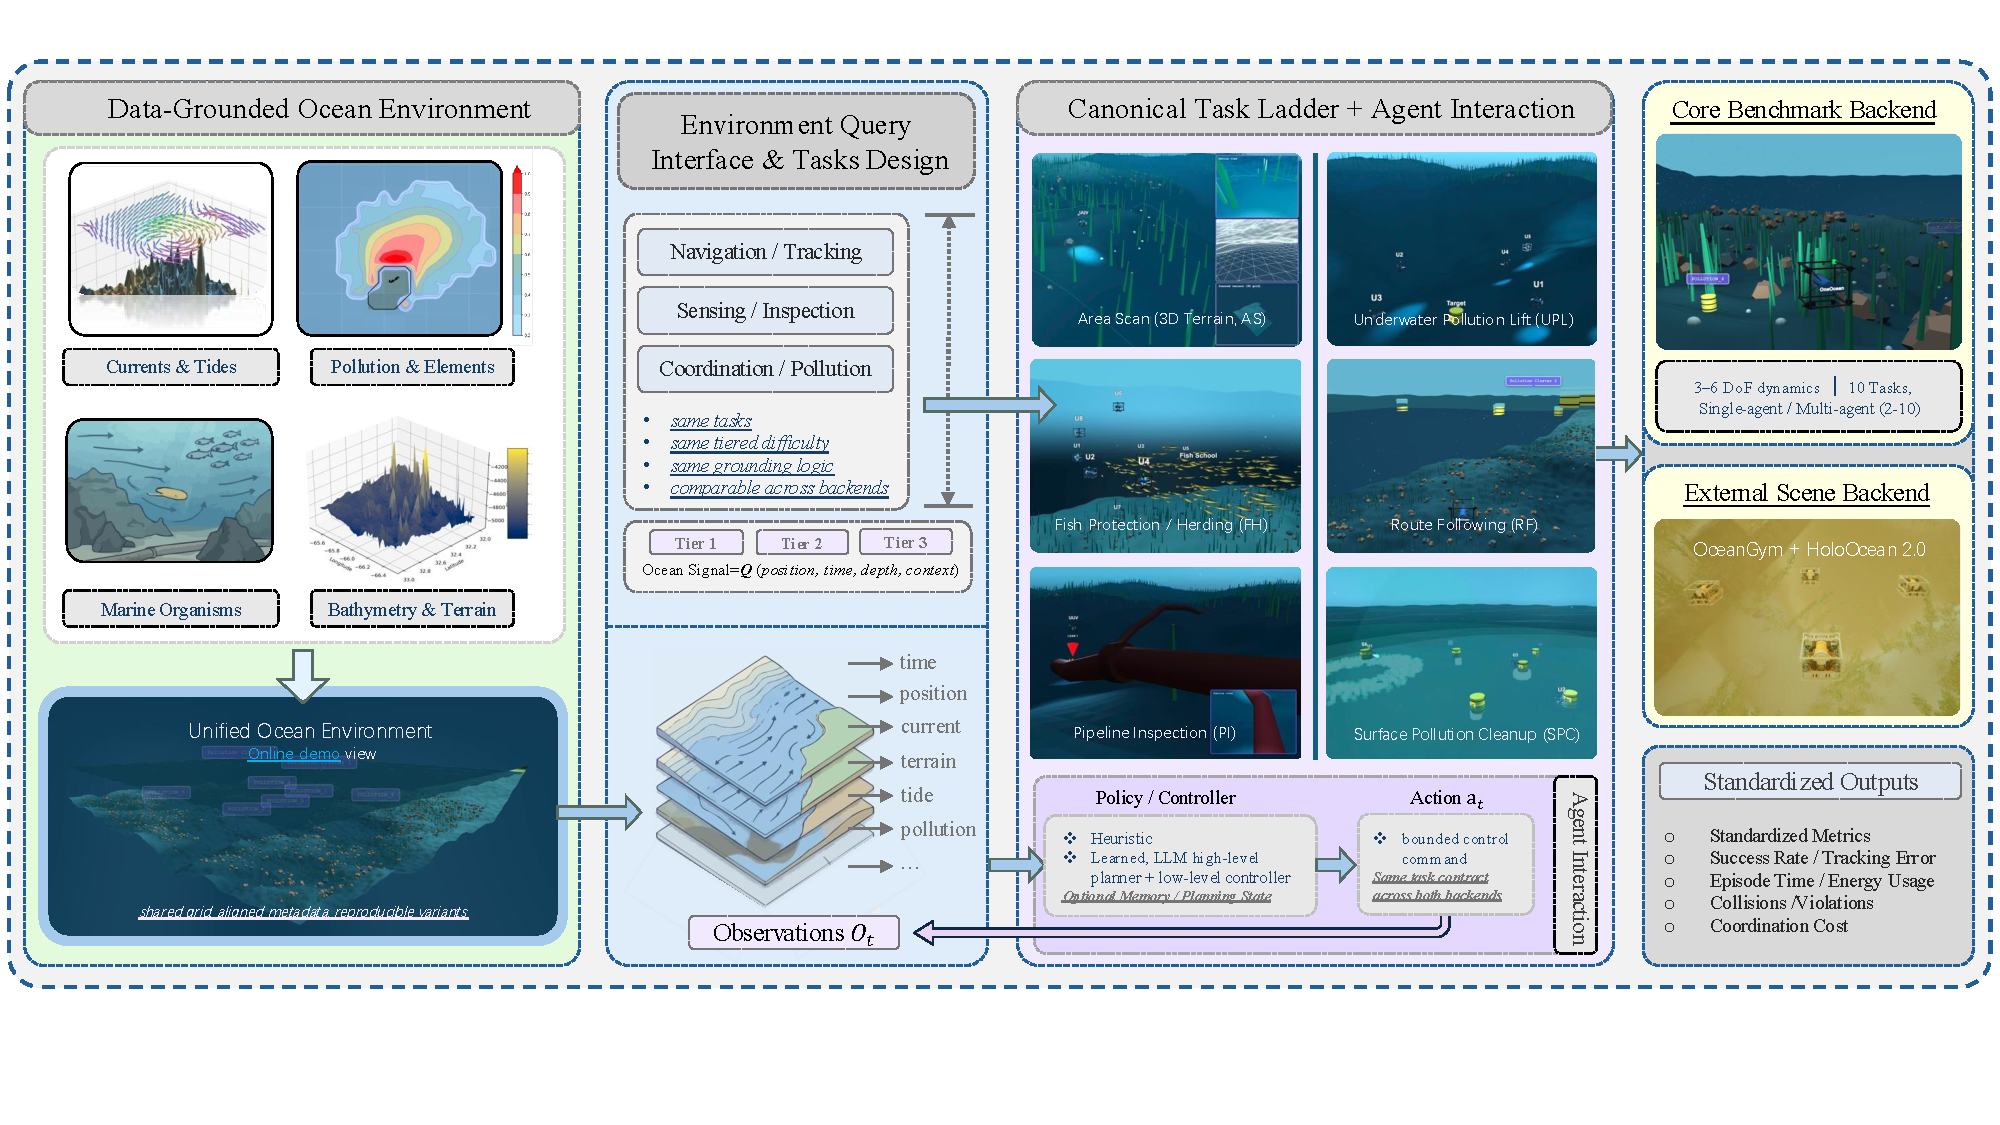
\includegraphics[width=0.99\textwidth]{figures/abstract.pdf}
    \caption{OneOcean overview. A shared ocean dataset supplies two simulation backends and a ten-task benchmark covering navigation, sensing, coordination, and pollution response.}
    \label{fig:overview}
\end{figure*}

\begin{abstract}
Simulation is essential for marine robotics, yet existing platforms often trade off visual realism, experimental throughput, and ocean conditions derived from real data. We present OneOcean, a data-grounded simulation suite and benchmark that combines bathymetry, currents, and tides in a shared spatiotemporal dataset. Optional pollution fields support pollution-response evaluation. OneOcean defines ten tasks covering navigation, sensing, coordination, and pollution response, with teams of 2--10 vehicles. The simulator supports three to six Degrees of Freedom (DoF) and records standardized metrics and run configurations across tasks, difficulty tiers, and team sizes. Experiments across dataset variants and underwater scenes compare heuristic control, Behavior Cloning (BC), and Large Language Model (LLM)-assisted planning under ocean currents.

\end{abstract}

\begin{links}
    \link{Project}{https://anonymous-2026.github.io/OneOcean/}
    \link{Code}{https://github.com/anonymous-2026/OneOcean}
    \link{Demo}{https://anonymous-2026.github.io/OneOcean/demo/}
\end{links}

% Scientific text is shared with the public paper; front matter stays anonymous.
\section{Introduction}

\revise{Marine robots must operate under complex, highly variable ocean conditions. In practice, \textbf{currents and tides} can dominate vehicle motion, while field trials remain expensive and time-limited and at-sea sensing and communication are constrained \cite{Trends_Marine_Robotics}. Simulation is therefore essential, but existing platforms often trade off between (i) visually realistic underwater worlds, (ii) high-throughput, reproducible experimentation, and (iii) \textbf{ocean-condition realism grounded in real data}.}

\revise{We present \textbf{OneOcean}, a data-grounded simulation suite and benchmark for marine robotics. OneOcean is built around a unified spatiotemporal ocean-environment dataset in Network Common Data Form (NetCDF). It harmonizes bathymetry from the General Bathymetric Chart of the Oceans (GEBCO) \cite{GEBCO2025} with data-driven currents and tides from the Copernicus Marine Service Global Ocean Physics Analysis and Forecast (GOPAF) product \cite{copernicus,CopernicusGOPAF2025}. OneOcean defines a \textbf{10-task benchmark} spanning single-agent navigation and tracking, spatial sensing and coverage, and multi-agent coordination and pollution-related tasks, with support for teams of 2--10 vehicles. The dataset variants support local iteration, scene construction, and public release under common task definitions. Figure~\ref{fig:overview} summarizes this organization.}

\begin{table*}[!t]
\centering
\scriptsize
\setlength{\tabcolsep}{0.6pt}
\renewcommand{\arraystretch}{1.02}
\textbf{Symbols:} \symyes\ Provided; \symno\ Not provided. \quad
\textbf{Tasks:} G2G, SK, RF, DPT, AS, PI, FT, SPC, UPL, and FH.\par
\begin{tabularx}{\textwidth}{@{}l c | *{9}{Y} *{10}{c}@{}}
\toprule
\textbf{Platform or Work} & \textbf{Venue}
& \makecell{\textbf{Real-data}\\ \textbf{In Loop}}
& \makecell{\textbf{Multi-}\\\textbf{agent}}
& \makecell{\textbf{Cross-}\\\textbf{backend}}
& \makecell{\textbf{3D}\\\textbf{Currents}}
& \makecell{\textbf{Pollution}\\\textbf{or Spill}}
& \makecell{\textbf{Tide}\\\textbf{Modeling}}
& \makecell{\textbf{Canonical}\\\textbf{Task}}
& \makecell{\textbf{Metrics}\\\textbf{Protocol}}
& \makecell{\textbf{Headless}\\\textbf{Batch}}
& \textbf{G2G} & \textbf{SK} & \textbf{RF} & \textbf{DPT} & \textbf{AS} & \textbf{PI} & \textbf{FT} & \textbf{SPC} & \textbf{UPL} & \textbf{FH} \\
\midrule

MIMIR-UW & 2023
& \symno & \symno & \symno
& \symno & \symno & \symno & \symno & \symno
& \symyes
& \symno & \symno & \symno & \symno & \symno & \symno & \symno & \symno & \symno & \symno \\

HoloOcean 2.0 & 2025
& \symno & \symyes & \symno
& \symyes & \symno & \symno & \symno & \symno
& \symyes
& \symyes & \symyes & \symyes & \symyes & \symyes & \symyes & \symyes & \symno & \symno & \symno \\

OceanSim & 2025
& \symno & \symyes & \symno
& \symno & \symno & \symno & \symno & \symno
& \symyes
& \symyes & \symno & \symyes & \symno & \symno & \symyes & \symyes & \symno & \symno & \symno \\

MarineGym & IROS 2025
& \symno & \symyes & \symyes
& \symyes & \symyes & \symyes & \symyes & \symyes
& \symyes
& \symyes & \symyes & \symyes & \symno & \symno & \symno & \symyes & \symno & \symno & \symno \\

OceanGym & 2025
& \symno & \symyes & \symyes
& \symyes & \symyes & \symno & \symyes & \symyes
& \symyes
& \symyes & \symyes & \symyes & \symno & \symyes & \symno & \symyes & \symno & \symno & \symno \\

URLab & ICRA 2026
& \symno & \symno & \symyes
& \symno & \symno & \symno & \symno & \symyes
& \symno
& \symyes & \symno & \symno & \symno & \symno & \symno & \symno & \symno & \symno & \symno \\

DREAM & ICRA 2026
& \symno & \symno & \symno
& \symno & \symno & \symno & \symno & \symyes
& \symno
& \symno & \symno & \symno & \symno & \symyes & \symyes & \symno & \symno & \symno & \symno \\

Douro MARL & ICRA 2026
& \symyes & \symyes & \symno
& \symno & \symyes & \symyes & \symno & \symyes
& \symyes
& \symno & \symno & \symno & \symno & \symyes & \symno & \symno & \symno & \symno & \symno \\

Map-TIDAL & ICRA 2026
& \symno & \symyes & \symno
& \symno & \symno & \symno & \symno & \symyes
& \symno
& \symno & \symno & \symno & \symno & \symyes & \symyes & \symno & \symno & \symno & \symno \\

CAMAR & AAAI 2026
& \symno & \symyes & \symno
& \symno & \symno & \symno & \symyes & \symyes
& \symyes
& \symyes & \symno & \symno & \symno & \symno & \symno & \symno & \symno & \symno & \symno \\

RobotArena $\infty$ & ICLR 2026
& \symyes & \symno & \symno
& \symno & \symno & \symno & \symyes & \symyes
& \symyes
& \symno & \symno & \symno & \symno & \symno & \symno & \symno & \symno & \symno & \symno \\

CaP-X & ICML 2026
& \symno & \symno & \symyes
& \symno & \symno & \symno & \symyes & \symyes
& \symyes
& \symno & \symno & \symno & \symno & \symno & \symno & \symno & \symno & \symno & \symno \\

\rowcolor{gray!20}%
\textbf{OneOcean (ours)} & 2026
& \symyes & \symyes & \symyes
& \symyes & \symyes & \symyes & \symyes & \symyes
& \symyes
& \symyes & \symyes & \symyes & \symyes & \symyes & \symyes & \symyes & \symyes & \symyes & \symyes \\

\bottomrule
\end{tabularx}
\caption{System-level comparison and task coverage. Entries are compiled from the cited papers and public documentation \cite{MIMIRUW,HoloOcean2,OceanSim,MarineGym,OceanGym,URLab2026,DREAM2026,DouroMARL2026,MapTIDAL2026,CAMAR2026,RobotArena2026,CaPX2026}.}
\label{tab:platform_features_tasks}
\end{table*}

\revise{OneOcean provides two complementary execution backends that share task definitions and evaluation semantics. The \emph{core benchmark backend} runs deterministic episodes at scale and records standardized metrics and run configurations. The \emph{external underwater-scene backend} runs the same tasks in packaged underwater scenes from an existing simulator using OneOcean current exports.}
In summary, our contributions are:
\begin{itemize}
    \item \revise{A shared ocean-environment dataset and tools for exporting currents to simulators, with variants for fast iteration, scene construction, and public release.}
    \item \revise{A 10-task benchmark with difficulty tiers, standardized metrics, reproducible run records, and 3--6 DoF vehicle dynamics, with 6DoF used for the main quantitative evaluation.}
    \item \revise{Experiments across the two backends that reveal task difficulty, scaling, and planner-compute trade-offs under data-grounded disturbances.}
\end{itemize}

\section{Related Work}
\label{sec:related_work}

Classical simulators built on Gazebo \cite{Gazebo}, including UUV Simulator \cite{UUVSim} and UWSim \cite{UWSim}, provide dynamics and sensor stacks for robotics workflows. More recent systems target higher-fidelity rendering or higher-throughput experimentation, including MARUS \cite{MARUS}, OceanSim on Isaac Sim \cite{OceanSim,IsaacSim}, DAVE \cite{DAVE}, MarineGym \cite{MarineGym}, and URLab, which integrates Unreal Engine with MuJoCo \cite{URLab2026}. \revise{OneOcean supplies a shared ocean dataset, a ten-task benchmark, and a reporting protocol across two execution backends. Table~\ref{tab:platform_features_tasks} compares system capabilities and task coverage.}

Ocean-condition realism is commonly provided by numerical models and operational forecasting systems. Representative community models include Delft3D \cite{delft3d}, NEMO \cite{nemo}, MITgcm \cite{MITgcm}, ROMS \cite{roms}, and HYCOM \cite{hycom}. Operational products from the Copernicus Marine Service, including GOPAF, provide data-assimilative currents and hydrographic variables. GEBCO provides global gridded seafloor elevation, while NetCDF stores labeled multidimensional coordinates, variables, units, and provenance in a self-describing representation. These sources are public, globally scoped, and machine-queryable, allowing the same ocean condition to be extracted and reproduced across runs. Toolkits such as Parcels \cite{parcels} and OpenDrift \cite{opendrift} support Lagrangian drift and dispersion analysis. \revise{OneOcean uses these ocean data sources to define reproducible robotics tasks across simulation backends.}

\revise{Recent marine-robotics studies address monitoring, inspection, and plume mapping. DREAM studies vision-language monitoring through simulation and tank trials \cite{DREAM2026}; Map-TIDAL allocates cooperative underwater-inspection tasks \cite{MapTIDAL2026}; and Douro MARL maps a data-driven river plume with multiple vehicles \cite{DouroMARL2026}. Recent robotics benchmarks evaluate multi-agent routing and transferable control. CAMAR defines high-throughput continuous multi-agent routing and a three-tier protocol \cite{CAMAR2026}; RobotArena $\infty$ converts real demonstrations into scalable simulation tests for robot policies \cite{RobotArena2026}; and CaP-X evaluates executable embodied agents across multiple manipulation suites \cite{CaPX2026}. OneOcean combines marine task definitions with ocean data, reproducible run records, and a common evaluation protocol across two backends.}

\section{OneOcean Suite}
\label{sec:oneocean_suite}

OneOcean combines a shared ocean dataset, two simulation backends, and a ten-task evaluation protocol.

\subsection{Unified spatiotemporal ocean dataset}
\label{sec:env_product}

The shared NetCDF representation harmonizes GEBCO bathymetry with GOPAF currents and optional tides. It exposes named latitude, longitude, time, and depth coordinates, eastward and northward current components, elevation, and a mask for invalid terrain and NoData cells. The pipeline crops the requested region, retains the returned time and depth levels, aligns variables on one horizontal grid, and records provenance.

The core backend selects a fixed $(t,d)$ slice for deterministic rollouts, whereas the external backend advances a dataset clock. Table~\ref{tab:data_variants} reports the realized products: the 0--200\,m requests returned 26 levels through 186.13\,m, while \texttt{tiny} contains one near-surface level at 0.494\,m. Appendix Sec.~\ref{supp-app:data} specifies the full schema, mask semantics, coordinate conventions, validation results, and tide sampling and depth treatment.

The validity mask marks unusable cells. The tide-enabled \texttt{scene} variant aligns tide samples to the dataset clock and applies depth attenuation.

\begin{table}[!t]
\centering
\scriptsize
\setlength{\tabcolsep}{2.2pt}
\renewcommand{\arraystretch}{1.08}
\begin{tabularx}{\columnwidth}{@{}l>{\raggedright\arraybackslash}p{0.30\columnwidth}>{\centering\arraybackslash}p{0.24\columnwidth}>{\raggedright\arraybackslash}X@{}}
\toprule
\textbf{Variant} & \textbf{Region and period} & \textbf{$T\!\times\!D\!\times\!H\!\times\!W$} & \textbf{Resolution; size; use} \\
\midrule
\texttt{tiny} & 42.1--42.7 N, 71.2--70.2 W; 2025 & $357\!\times\!1\!\times\!62\!\times\!101$ & $\approx0.01^\circ$; 29 MB; tests and web \\
\texttt{scene} & 32--33 N, 66.5--65.5 W; Dec. 2025 & $23\!\times\!26\!\times\!240\!\times\!240$ & $0.00418^\circ$; 690 MB; scenes \\
\texttt{public} & 30--40 N, 72--62 W; 2025 & $357\!\times\!26\!\times\!41\!\times\!41$ & $0.25^\circ$; 175 MB; release \\
\bottomrule
\end{tabularx}
\caption{Realized combined NetCDF variants. Sizes are the merged products themselves; source subsets and derived assets are distributed separately.}
\label{tab:data_variants}
\end{table}

\subsection{Data-grounded disturbance signals}
\label{sec:signals}

OneOcean exports either a fixed gridded slice for high-throughput rollouts or a temporal profile for scene-backed execution. Both apply current through a recorded relative-velocity convention in the core frame $(x,y,z)=$(east, depth-down, north), and every artifact records its extraction indices. Figure~\ref{fig:base_current_field} shows one current slice over bathymetry; Appendix Sec.~\ref{supp-app:data} details sampling, export, and provenance.

\begin{figure}[t]
 \centering
 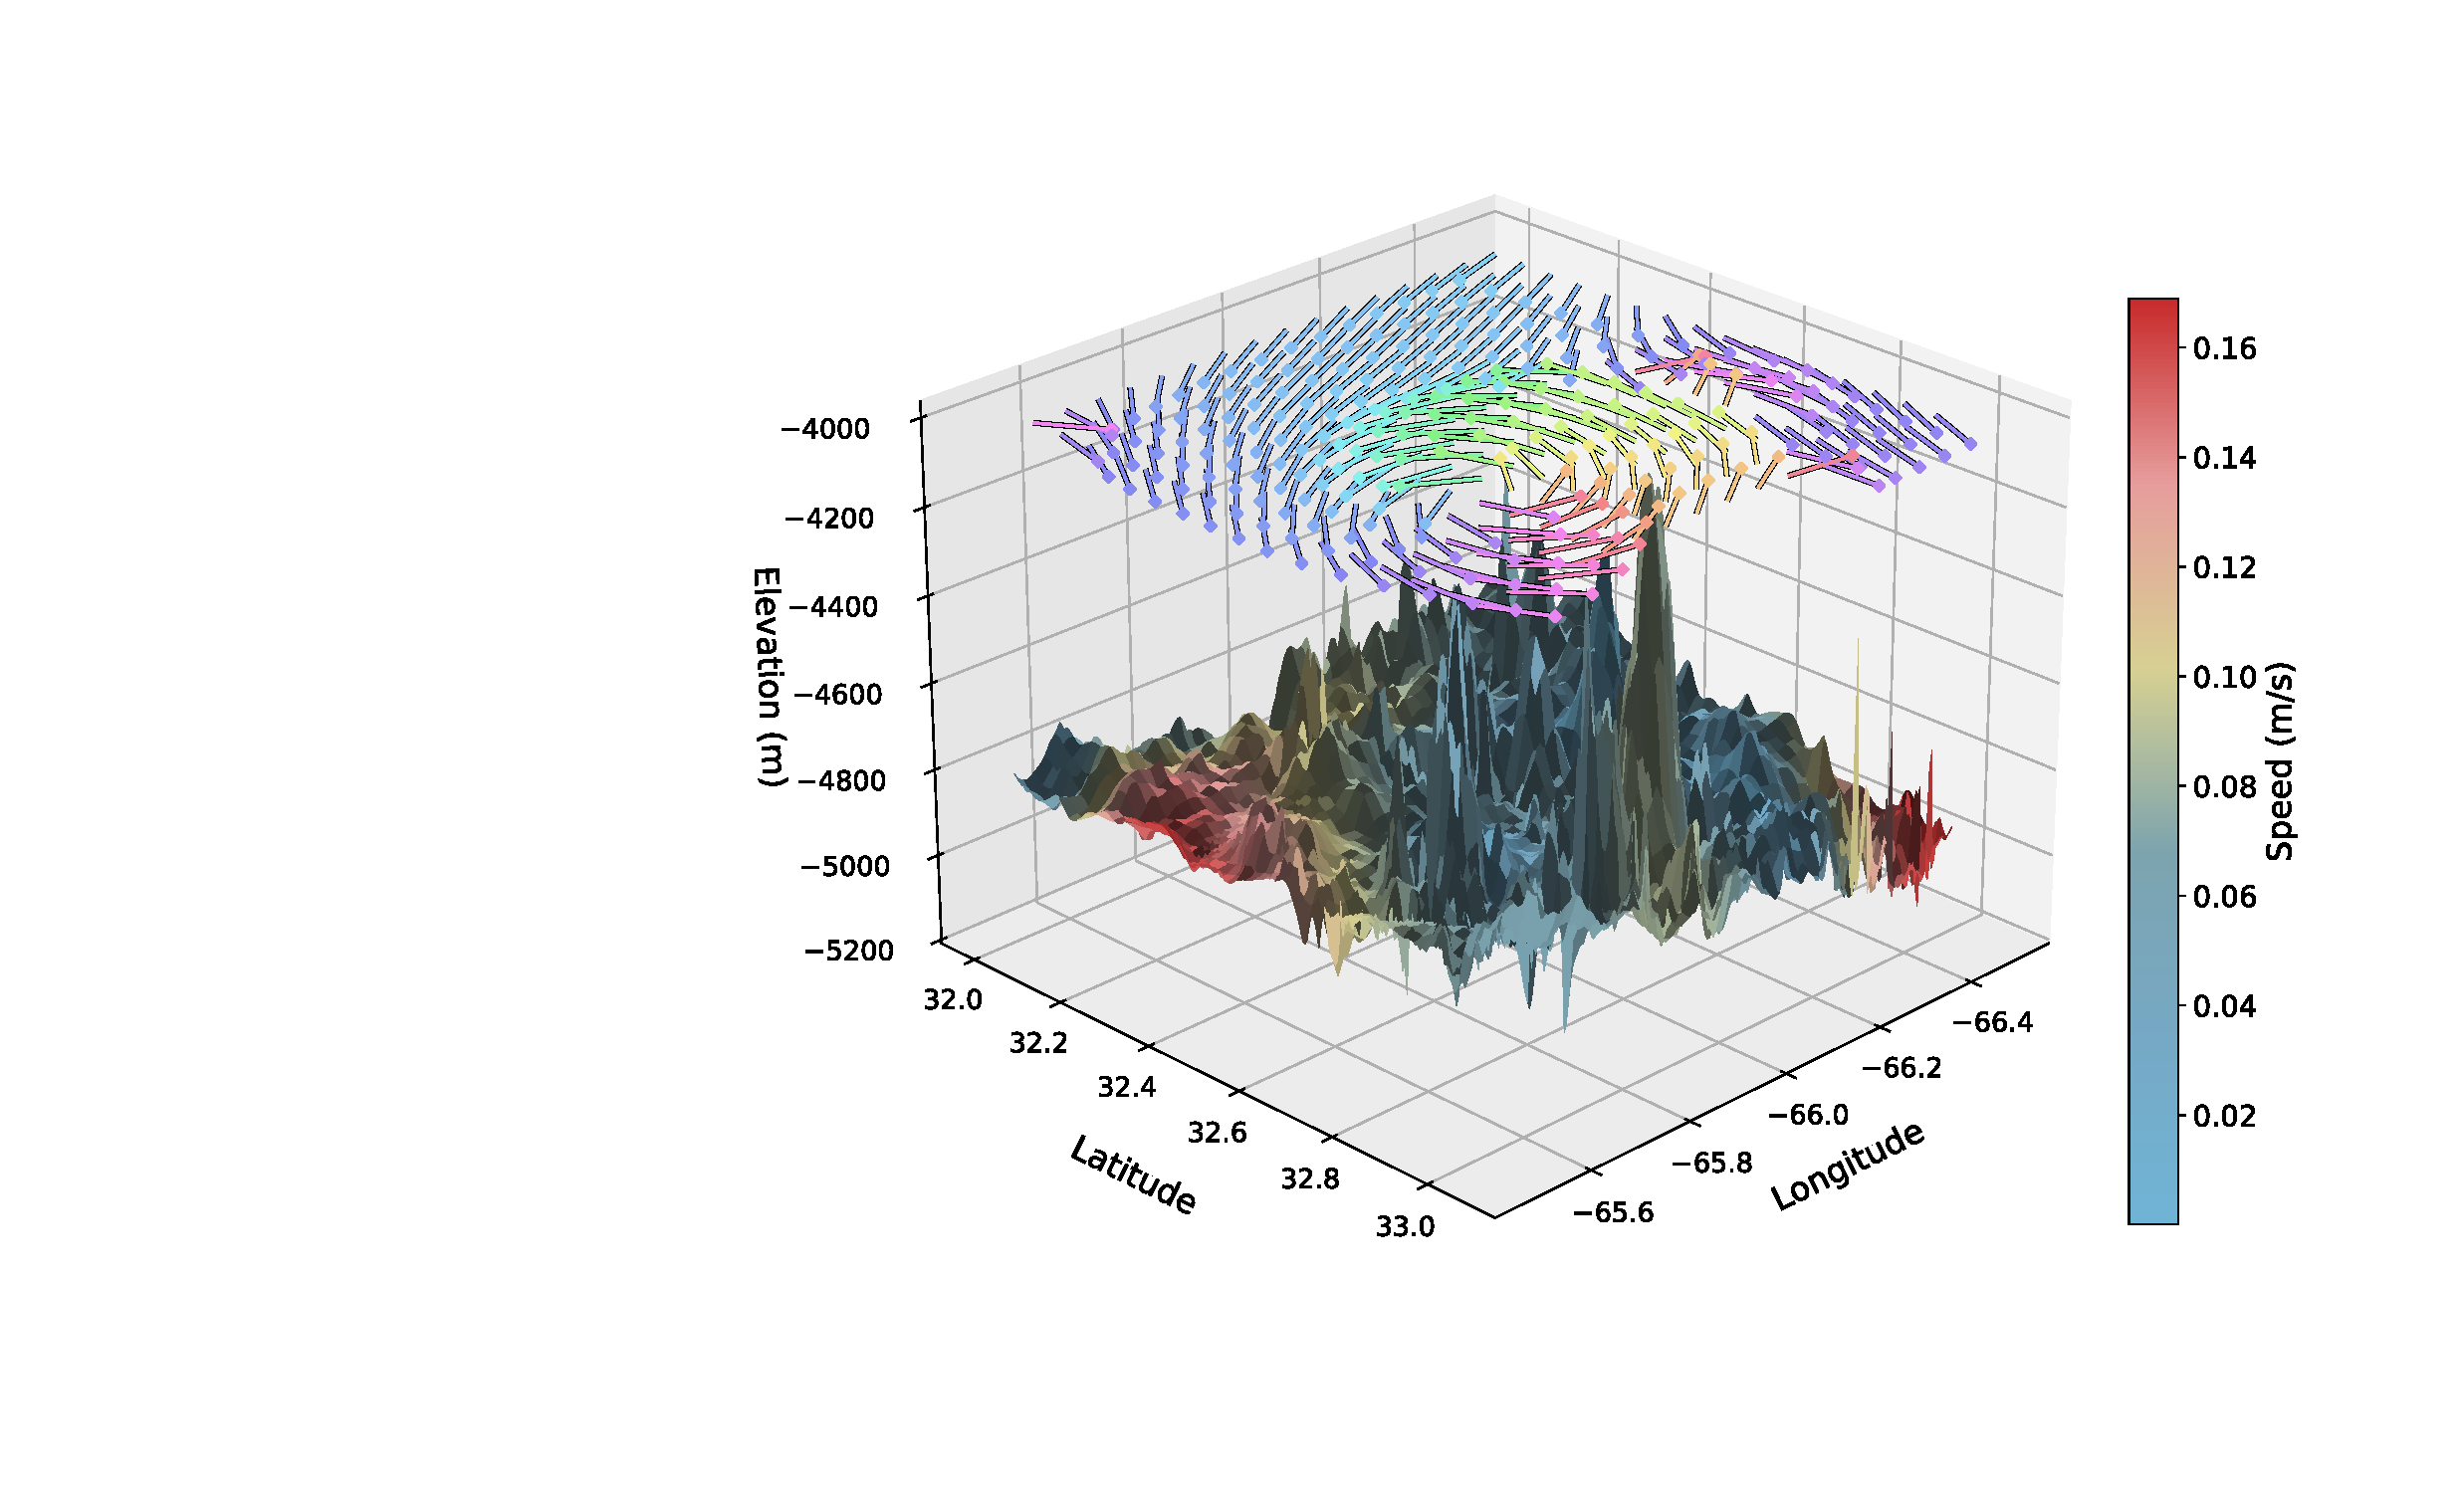
\includegraphics[width=0.98\linewidth]{figures/ocpnet_base_current_3d_diffusion_el25_az045.pdf}
 \caption{Base current field visualization over bathymetry. The horizontal current components are $u_{\mathrm{data}}$ and $v_{\mathrm{data}}$; surface color indicates speed magnitude (m\,s$^{-1}$). View configuration: pitch $25^\circ$, azimuth $45^\circ$, and depth index $0$ (source depth 0.494\,m). The terrain surface is colored by speed and overlaid with arrows indicating current direction.}
 \label{fig:base_current_field}
\end{figure}

\paragraph{Environment queries and probes.}
\label{sec:queries_probes}

Shared queries expose local current, bathymetry, mask validity, and task signals. Pollution tasks observe $o_i^c(t)=C(p_i(t),t)$ from either a current-advected Gaussian or an Ocean Current Prediction Network (OCPNet) field. Both models generate reproducible synthetic concentration signals. Appendix Sec.~\ref{supp-app:models_ros} gives the probe, sink, and discrete-source cleanup semantics.

\subsection{Task suite and difficulty tiers}
\label{sec:tasks}

OneOcean defines ten tasks spanning navigation and tracking (G2G, SK, RF, DPT), sensing and inspection (AS, PI), and coordination and pollution response (FT, SPC, UPL, FH). Table~\ref{tab:task_ladder} gives team sizes and primary metrics; Appendix Sec.~\ref{supp-app:tasks} provides the complete objectives, observations, constraints, and success conditions.

\begin{table}[!t]
\centering
\scriptsize
\setlength{\tabcolsep}{3pt}
\renewcommand{\arraystretch}{1.08}
\begin{tabular*}{\columnwidth}{@{\extracolsep{\fill}}>{\raggedright\arraybackslash}p{0.18\columnwidth}c c c >{\raggedright\arraybackslash}p{0.28\columnwidth}@{}}
\toprule
\textbf{Category} & \textbf{Task} & \textbf{Agents} & \textbf{Goal} & \textbf{Primary metric} \\
\midrule
Navigation & \textbf{G2G} & 1 & reach & final goal error \\
Navigation & \textbf{SK} & 1 & hold & station root-mean-square error \\
Navigation & \textbf{RF} & 1 & follow & cross-track error \\
Navigation & \textbf{DPT} & 1 & track & depth-tracking error \\
\makecell[l]{Sensing and\\Coverage} & \textbf{AS} & 1--10 & scan & coverage fraction \\
\makecell[l]{Sensing and\\Inspection} & \textbf{PI} & 1--10 & inspect & inspection score \\
Coordination & \textbf{FT} & 2--10 & transit & formation error \\
Pollution & \textbf{SPC} & 2--10 & clean & cleanup rate \\
Coordination & \textbf{UPL} & 5 & lift & lift success \\
Coordination & \textbf{FH} & 8 & herd & containment success \\
\bottomrule
\end{tabular*}
\caption{The OneOcean task suite (10 tasks). Each task is evaluated at Tiers 1--3 and paired with a compact goal type and a primary task-specific metric.}
\label{tab:task_ladder}
\end{table}

\revise{Tiers 1, 2, and 3 jointly increase current strength, precision, route and coverage extent, sensing difficulty, and coordination tightness while preserving each task's interface. Every task declares its objective, observations, feasibility constraints, success condition, and primary metric. The release also includes a lightweight Robot Operating System 2 (ROS~2) bridge for state, probes, and velocity commands; its frames, topics, services, and interface checks appear in Appendix Sec.~\ref{supp-app:models_ros}.}

Navigation and tracking tasks test disturbance rejection and sustained trajectory accuracy; sensing and inspection tasks require spatial coverage or physical cue encounters; coordination and pollution tasks add team geometry, assignment, and dwell-time coupling. We report success together with task-specific progress.

\revise{
\begin{table*}[!t]
\centering
\scriptsize
\setlength{\tabcolsep}{1.2pt}
\renewcommand{\arraystretch}{1.10}
\begin{tabularx}{\textwidth}{@{}l*{3}{Y}|*{3}{Y}|*{6}{Y}@{}}
\toprule
\multirow{2}{*}{\textbf{Method}} & \multicolumn{3}{c}{\textbf{Macro (Tier 2)}} & \multicolumn{3}{c}{\textbf{Macro (Tier 3)}} & \multicolumn{6}{c}{\textbf{Tier 3 key-task metrics}} \\
\cmidrule(lr){2-4}\cmidrule(lr){5-7}\cmidrule(lr){8-13}
 & \makecell{Suite\\SR(\%)} & \textbf{$E$} & \makecell{Coll.\\(\%)} & \makecell{Suite\\SR(\%)} & \textbf{$E$} & \makecell{Coll.\\(\%)} & \makecell{G2G\\SR(\%)} & \makecell{RF\\SR(\%)} & \makecell{SK\\RMS} & \makecell{Scan\\cov.} & \makecell{Pipe\\score} & \makecell{Cleanup\\rate} \\
\midrule
\rowcolor{oursbg}
Heuristic & \best{84.6} & 1842.3 & \best{5.68} & \best{29.0} & 3352.4 & 8.19 & \best{74.0} & \best{54.0} & \best{1.07} & \best{0.89} & \best{0.78} & \best{0.56} \\
BC & 58.6 & \best{1271.2} & 9.72 & 6.0 & \best{1635.1} & \best{6.41} & 34.0 & 0.0 & 26.52 & 0.89 & 0.67 & 0.06 \\
\bottomrule
\end{tabularx}
\caption{Headline core-benchmark results (6DoF): macro averages at Tiers 2 and 3 plus Tier 3 key-task metrics, using 50 episodes per task and tier. Success Rate (SR) is reported in percent; Macro Suite SR is an unweighted mean across the 10 tasks. Coll is the mean collision-step ratio (\%) with a 2.0\,m radius. Best values per column are highlighted.}
\label{tab:headline_macro_keymetrics}
\end{table*}
}

\revise{
\begin{table*}[t]
\centering
\scriptsize
\setlength{\tabcolsep}{1.5pt}
\renewcommand{\arraystretch}{1.10}
\begin{tabularx}{\textwidth}{@{}l*{9}{Y}@{}}
\toprule
\textbf{Method} & \makecell{Avg.\\SR(\%)} & \makecell{Cleanup\\SR(\%)} & \makecell{Cleanup\\rate} & \makecell{Scan\\SR(\%)} & \makecell{Scan\\cov.} & \makecell{Pipe\\SR(\%)} & \makecell{Pipe\\score} & \textbf{$T$(s)} & \textbf{$E$} \\
\midrule
\rowcolor{oursbg}
Heuristic & \best{65.8} & 60.0 & \best{0.87} & \best{77.5} & 0.80 & \best{60.0} & \best{0.69} & \best{776.8} & 9132.4 \\
BC & 45.0 & 10.0 & 0.32 & 67.5 & 0.79 & 57.5 & 0.61 & 921.6 & \best{6908.2} \\
LLM-ChatGLM3-6B & 55.0 & 60.0 & \best{0.87} & 77.5 & \best{0.82} & 27.5 & 0.54 & 860.3 & 9671.5 \\
LLM-Qwen2.5-7B & 47.5 & 57.5 & 0.81 & 57.5 & 0.78 & 27.5 & 0.57 & 1077.2 & 11703.8 \\
LLM-Qwen2-7B & 45.0 & 57.5 & 0.86 & 67.5 & 0.81 & 10.0 & 0.51 & 991.4 & 10422.1 \\
LLM-Mistral-7B & 42.5 & 55.0 & 0.82 & 55.0 & 0.78 & 17.5 & 0.52 & 1044.2 & 11288.9 \\
LLM-Llama3-8B & 44.2 & \best{67.5} & 0.84 & 47.5 & 0.77 & 17.5 & 0.59 & 1099.1 & 11614.2 \\
LLM-Llama2-7B & 30.8 & 55.0 & \best{0.87} & 27.5 & 0.75 & 10.0 & 0.46 & 1156.4 & 11654.3 \\
\bottomrule
\end{tabularx}
\caption{Core-benchmark planning-suite performance at Tier 2 with doubled currents: heuristic vs BC vs local LLM planners on three planning-sensitive tasks, using 40 episodes per task (120 per method). Best values per column are highlighted.}
\label{tab:planning_suite_perf_t2}
\end{table*}
}


\subsection{Two execution backends}
\label{sec:backends}

The two backends share task definitions and reporting formats. The headless \textbf{core benchmark backend} consumes a NumPy Archive (NPZ) current slice and task and action configurations. It returns observations, metrics, run records, and recorder streams, and supports 3--6 DoF vehicle dynamics (6DoF in the main experiments) \cite{UUVSim}. The \textbf{external underwater-scene backend} runs the task suite in packaged underwater scenes using a temporal OneOcean current export. It returns route and task metrics alongside simulation recordings.

\paragraph{Benchmark protocol and metrics.}
\label{sec:protocol}

\begin{figure}[!b]
 \centering
 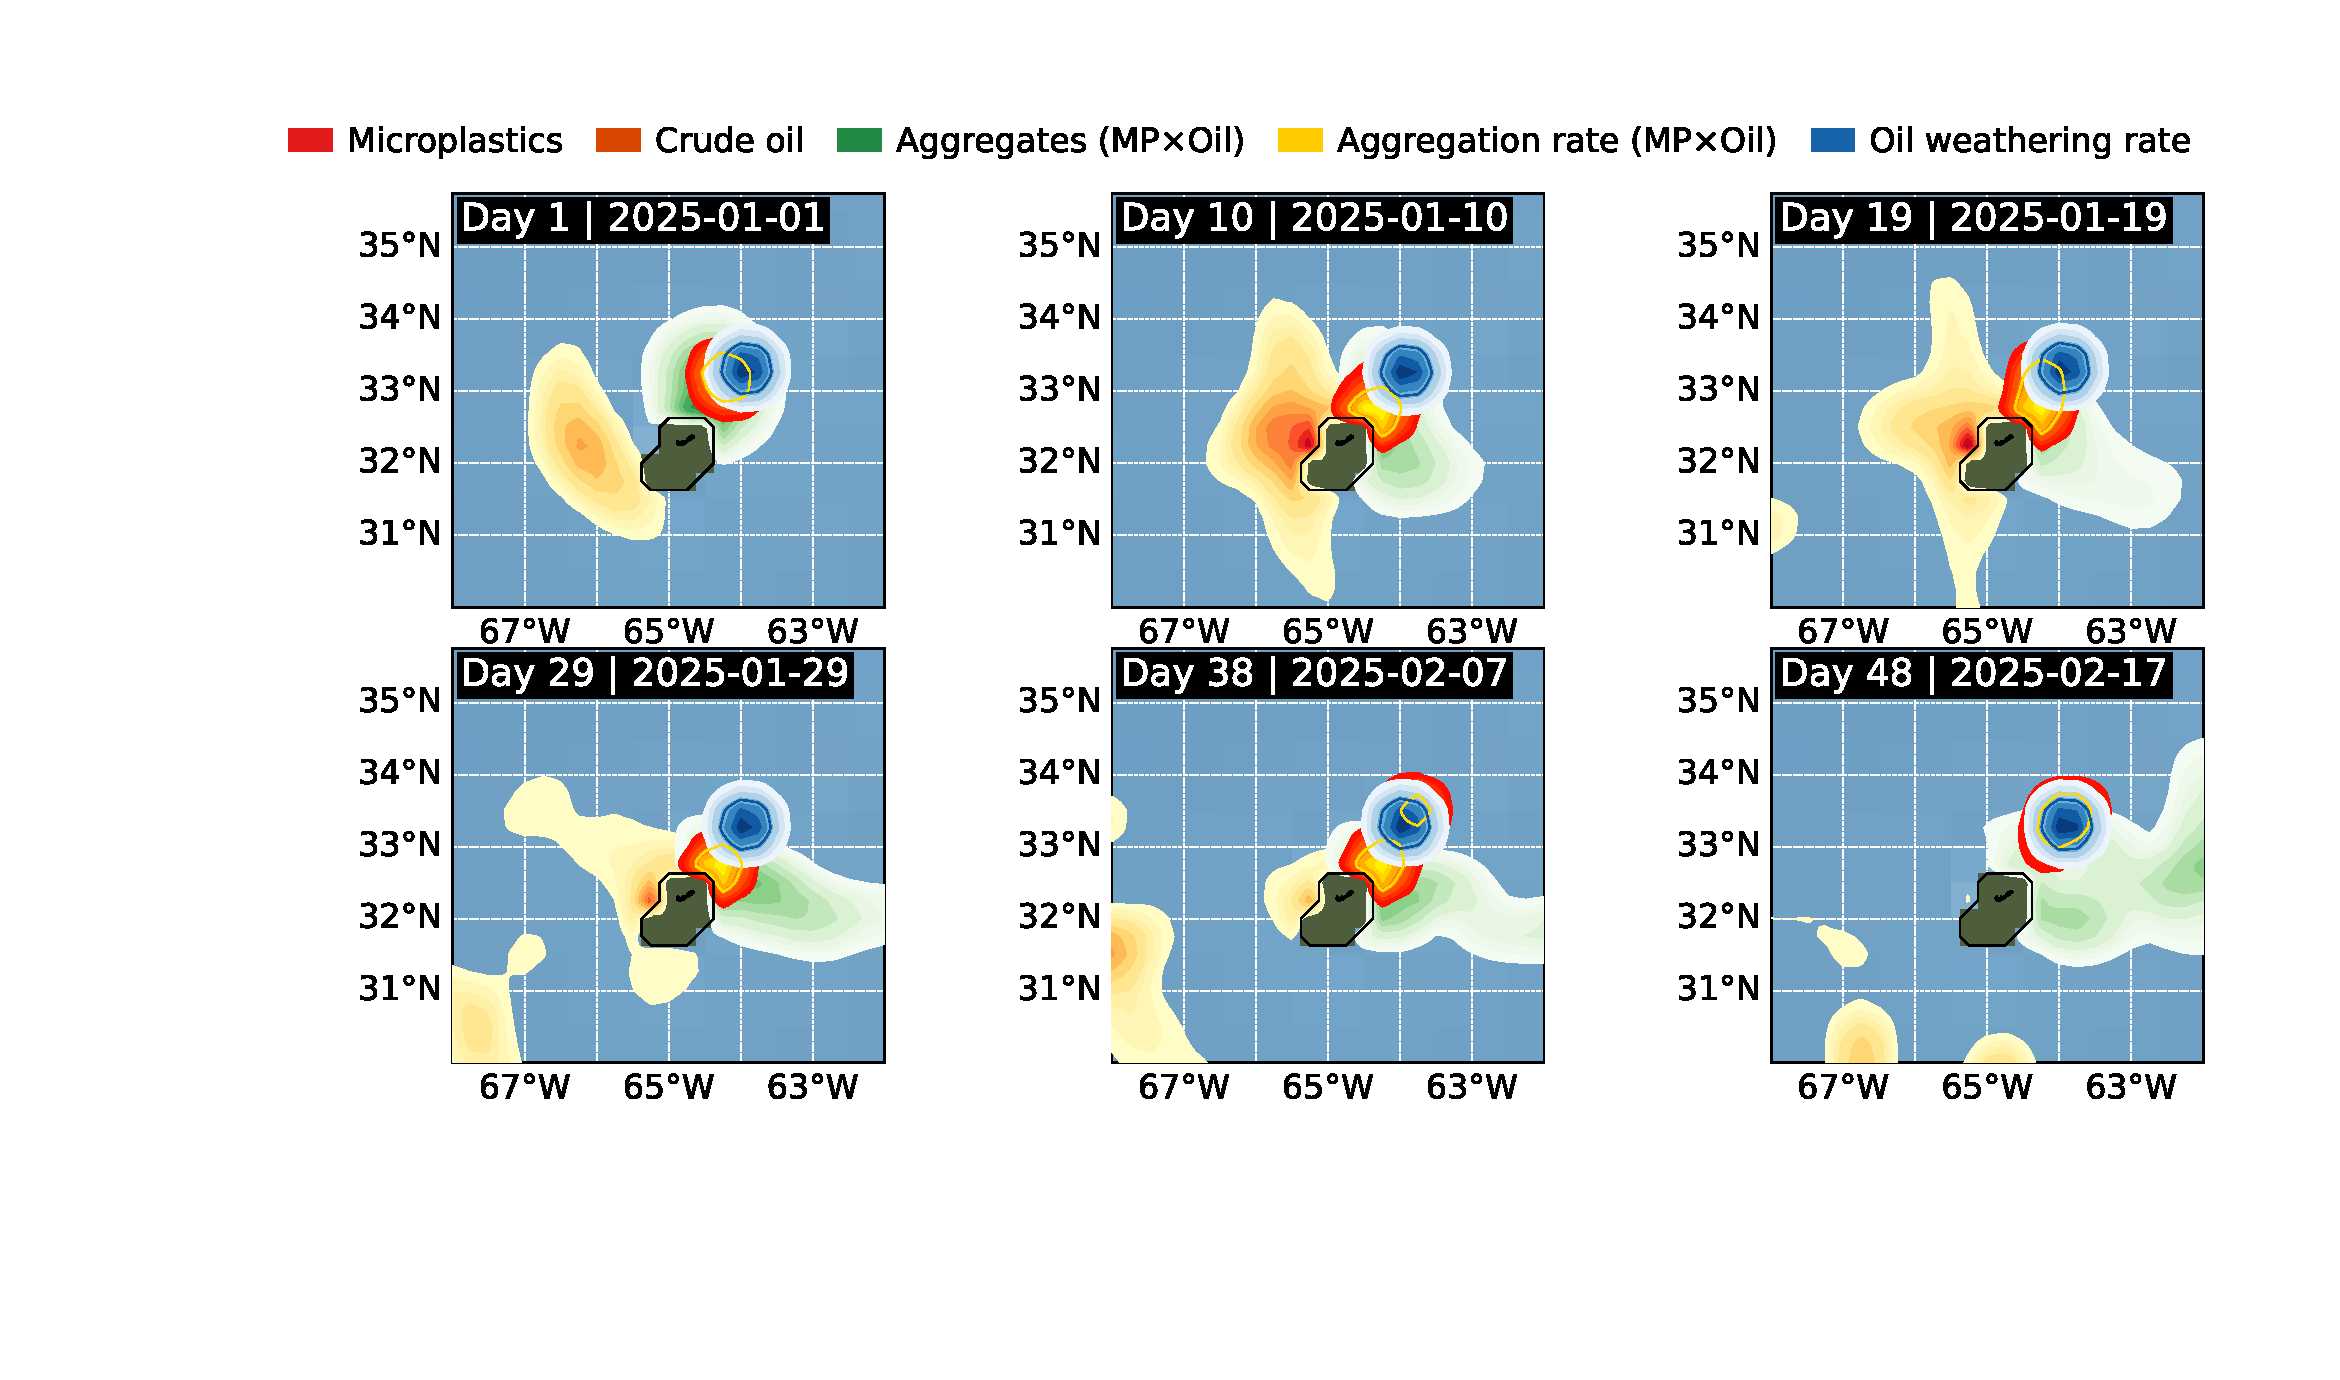
\includegraphics[width=0.98\linewidth]{figures/ocpnet_multispecies_seed04_panel.pdf}
 \caption{OCPNet multispecies diffusion and reaction fields that can generate concentration observations for localization, containment, and cleanup tasks.}
 \label{fig:ocpnet_panels}
\end{figure}

\revise{Actions specify desired relative velocity, clipped as $a_t=\mathrm{clip}(\tilde a_t;v_{\max})$. With current gain $g$,}
\begin{equation}
\revise{c_t = g\,[u_{\mathrm{data}}(x_t,z_t),\,0,\,v_{\mathrm{data}}(x_t,z_t)] + c_{\mathrm{tide}}(t),}
\end{equation}
\revise{where $u_{\mathrm{data}}$ and $v_{\mathrm{data}}$ are sampled horizontal currents and $c_{\mathrm{tide}}$ is an optional synthetic robustness signal. With body velocity $\nu=[\nu_\ell^\top,\nu_a^\top]^\top$, rotation $R$, and diagonal $M,D,K_\ell,K_a,K_d$, the diagonal 6DoF update is}
\begin{align}
M\dot\nu &= \tau-D\nu, &
\tau_\ell &= K_\ell(\nu_\ell^{\rm cmd}-\nu_\ell), \nonumber\\
\tau_a &= K_a(\nu_a^{\rm cmd}-\nu_a)-K_d\nu_a, &
\dot p &= R\nu_\ell+c_t .
\end{align}
\revise{Commands are transformed to the body frame; yaw follows horizontal motion while roll and pitch are stabilized. Kinematic mode directly integrates $a_t+c_t$, and 3DoF suppresses roll and pitch. The model uses diagonal inertia and damping, bounded attitude, and externally sampled current transport. Added mass, Coriolis and restoring terms, thruster allocation, and two-way fluid coupling are omitted. Hard terrain feasibility is}
\begin{equation}
\mathcal C=\{(x,y,z)\mid m_{\mathrm{land}}(x,z)<\tau_{\mathrm{land}},\ y+\delta_{\mathrm{clr}}\le-h(x,z)\},
\end{equation}
\revise{where $m_{\mathrm{land}}$ is mask validity, $h$ is bathymetric elevation, and $\delta_{\mathrm{clr}}$ is required clearance. Masked, out-of-bounds, or clearance-violating proposals are rejected through the shared constraint path. We report SR, timeout-aware episode time $T$, $E=\sum_t\|a_t\|_2^2\Delta t$, near-collision ratio, and task-specific metrics.}

\revise{BC maps normalized goal, depth, probe, current, and task features $\phi_t$ to $\hat a_t=f_\theta(\phi_t)$ and minimizes the heuristic-action loss}
\begin{equation}
\mathcal L_{\mathrm{BC}}=N_{\mathrm{BC}}^{-1}\sum_t\|a_t^{\mathrm{heur}}-\hat a_t\|_2^2.
\end{equation}
\revise{Every $K$ steps, an LLM instead proposes a discrete assignment $g_k=\pi_{\mathrm{LLM}}(s_k)$; schema-invalid output invokes a deterministic allocator, and a shared low-level controller executes $a_t=\pi_{\mathrm{low}}(x_t,g_k)$. Appendix Sec.~\ref{supp-app:models_ros} gives dynamics defaults, pollution semantics, and ROS mapping; Appendix Sec.~\ref{supp-app:protocol} defines all metrics and manifests.}

\paragraph{Optional pollution fields (OCPNet).}
\label{sec:ocpnet}

\revise{Continuous containment applies a local concentration sink. SPC completes discrete sources after an assignment-and-dwell condition; its cleanup rate is the fraction of sources completed. Figure~\ref{fig:ocpnet_panels} shows the multispecies concentration signal.}

\section{Experiments}
\label{sec:experiments}

\revise{We compare heuristic, BC, and LLM-assisted controllers across tasks, difficulty tiers, and team sizes, then evaluate task transfer to underwater scenes.}

\subsection{Experimental setup}

\revise{The main core results use 6DoF with hard mask and clearance checks and a fixed NetCDF-derived current slice; the external backend advances a temporal export in four packaged scenes. We report SR, timeout-aware $T$, action-energy proxy $E$, near-collision ratio, and the task metrics named in the tables. Episode budgets accompany each result table. Additional experiments examine planner decisions, dynamics sensitivity, and pollution observations. All runs store their integer seed, task and dynamics configuration, dataset indices, and software and Git state. Local LLM inference assigns one 48\,GB accelerator to each process. Appendix Sec.~\ref{supp-app:protocol} specifies the supplementary diagnostic budgets and recorded configuration fields.}

\revise{Here $T$ uses success time on successful episodes and timeout on failures; $E$ accumulates squared clipped vehicle commands over time. Coll(\%) counts steps in which the closest agent pair is within the configured near-collision radius. We also report coverage, inspection, source completion, station error, Cross-Track Error (CTE), and reached waypoints. Each of Tiers 1--3 jointly specifies disturbance, tolerance, spatial extent, and coordination settings.}

\subsection{Core benchmark backend}


\revise{
\begin{table}[!t]
\centering
\scriptsize
\setlength{\tabcolsep}{3.0pt}
\renewcommand{\arraystretch}{1.10}
\begin{tabularx}{\columnwidth}{@{}>{\raggedright\arraybackslash}p{0.21\columnwidth}c*{4}{Y}@{}}
\toprule
\textbf{Task} & \textbf{$N$} & \textbf{Heur T2} & \textbf{BC T2} & \textbf{Heur T3} & \textbf{BC T3} \\
\midrule
\rowcolor{scenarioGray}\multicolumn{6}{c}{\textit{Navigation and Tracking}} \\
\makecell[l]{G2G} & 1 & \best{94.0} & 44.0 & \best{74.0} & 34.0 \\
\makecell[l]{SK} & 1 & \best{100.0} & 0.0 & \best{14.0} & 0.0 \\
\makecell[l]{RF} & 1 & \best{84.0} & 24.0 & \best{54.0} & 0.0 \\
\makecell[l]{DPT} & 1 & \best{84.0} & 64.0 & \best{50.0} & 0.0 \\
\rowcolor{scenarioGray}\multicolumn{6}{c}{\textit{Coordination}} \\
\makecell[l]{FT} & 10 & \best{100.0} & 40.0 & \best{20.0} & 0.0 \\
\makecell[l]{FH} & 8 & 94.0 & \best{100.0} & 4.0 & \best{4.0} \\
\rowcolor{scenarioGray}\multicolumn{6}{c}{\textit{Sensing and Pollution}} \\
\rowcolor{oursbg}
\makecell[l]{PI} & 1 & \best{100.0} & 90.0 & \best{30.0} & 14.0 \\
\rowcolor{oursbg}
\makecell[l]{AS} & 1 & \best{90.0} & 84.0 & \best{14.0} & 4.0 \\
\rowcolor{oursbg}
\makecell[l]{SPC} & 10 & \best{84.0} & 50.0 & \best{10.0} & 0.0 \\
\rowcolor{oursbg}
\makecell[l]{UPL} & 5 & 16.0 & \best{90.0} & \best{20.0} & 4.0 \\
\bottomrule
\end{tabularx}
\caption{Per-task success rates at Tier 2 and Tier 3 for the 10-task suite, using 50 episodes per task and tier. Highlighted rows are revisited in the planning and external-backend transfer studies.}
\label{tab:per_task_sr_t2_t3}
\end{table}
}

\revise{
\begin{figure}[!t]
 \centering
 \subfloat[SPC: Surface Pollution Cleanup (multi-agent)]{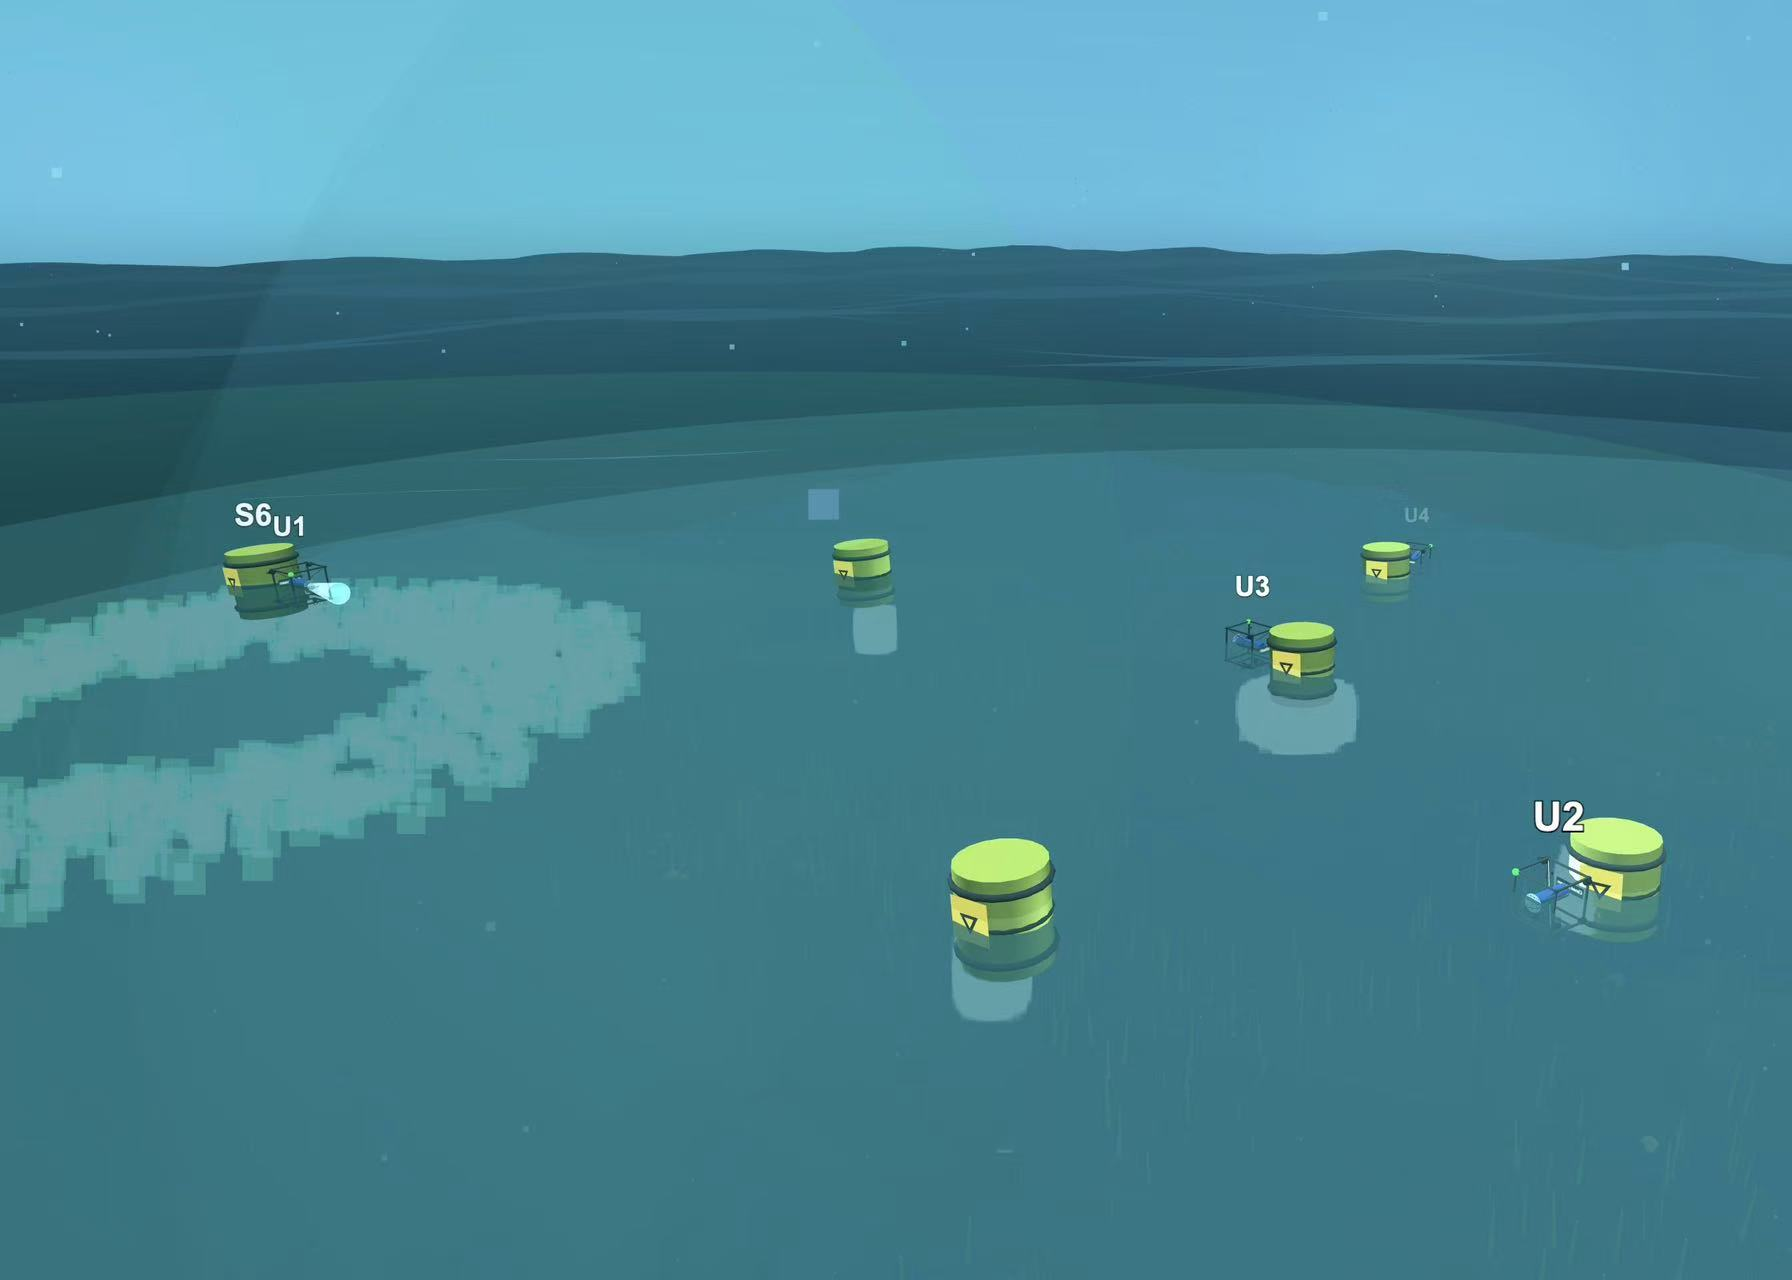
\includegraphics[width=0.48\linewidth]{figures/task1_ui_off.png}}
 \hfill
 \subfloat[UPL: Underwater Pollution Lift (5 UUVs)]{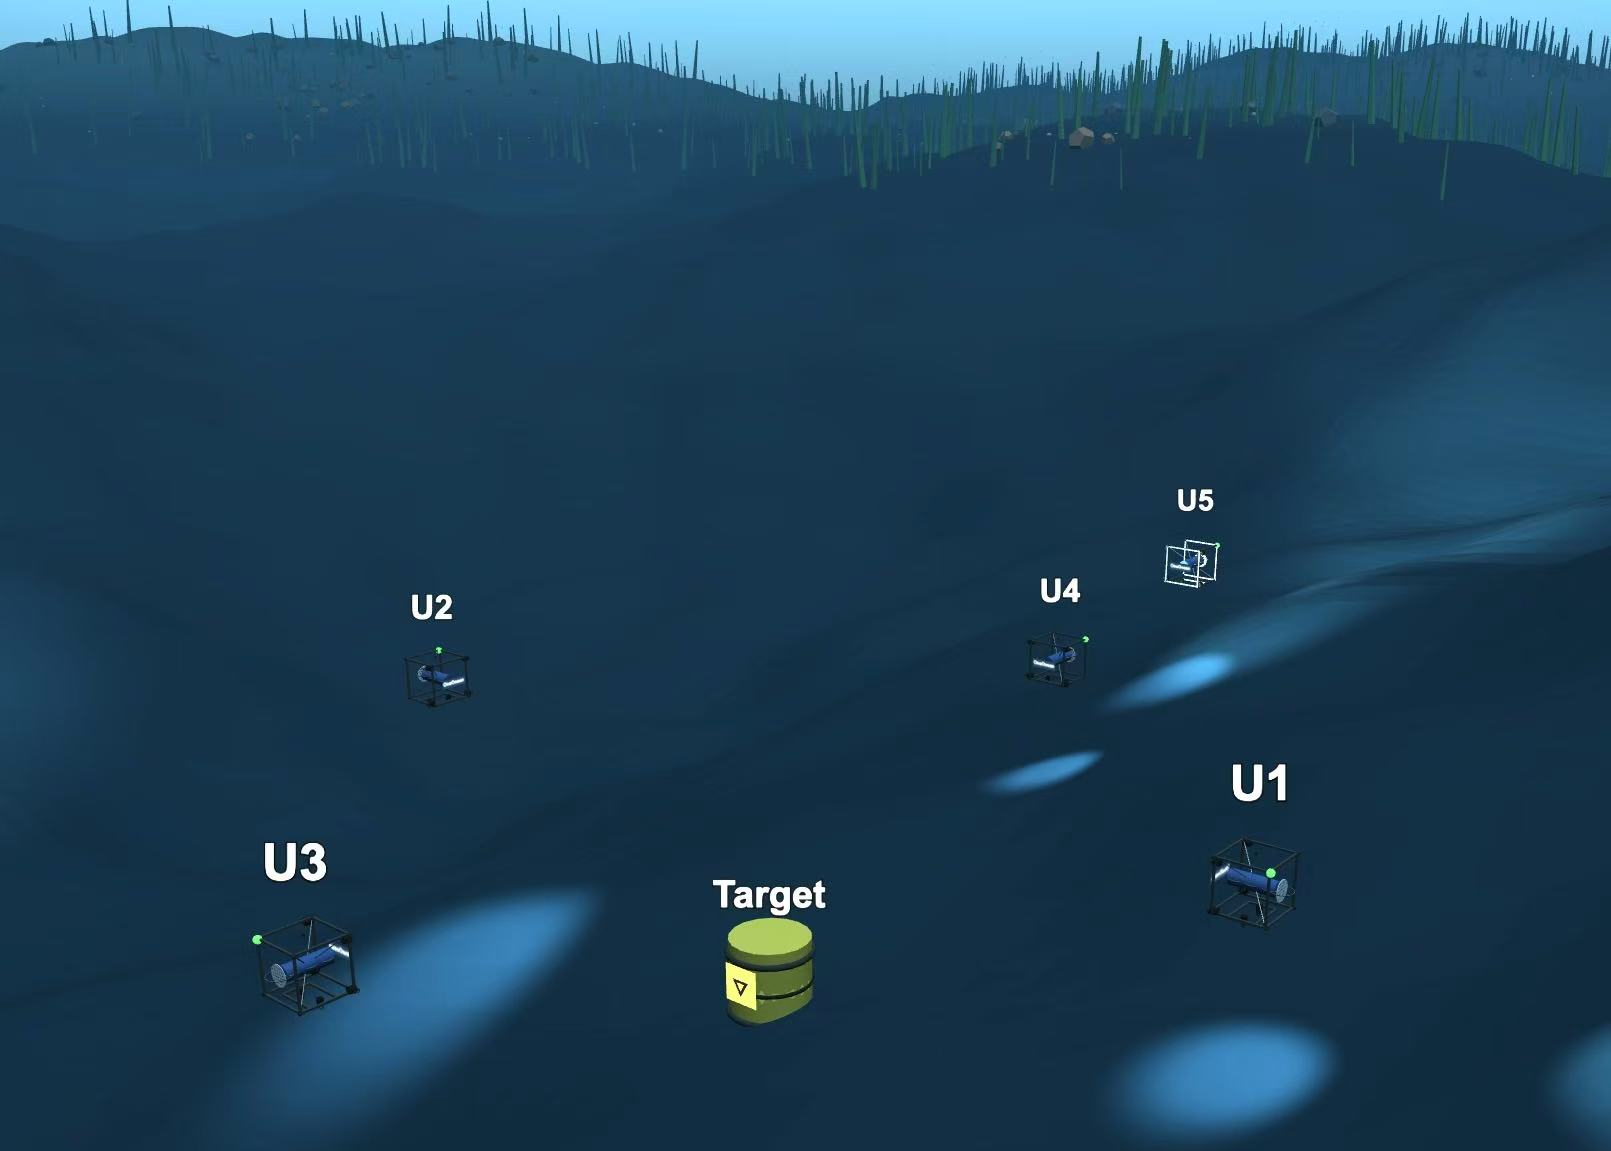
\includegraphics[width=0.48\linewidth]{figures/task2_ui_off.png}}\\
 \subfloat[AS: Area Scan over terrain]{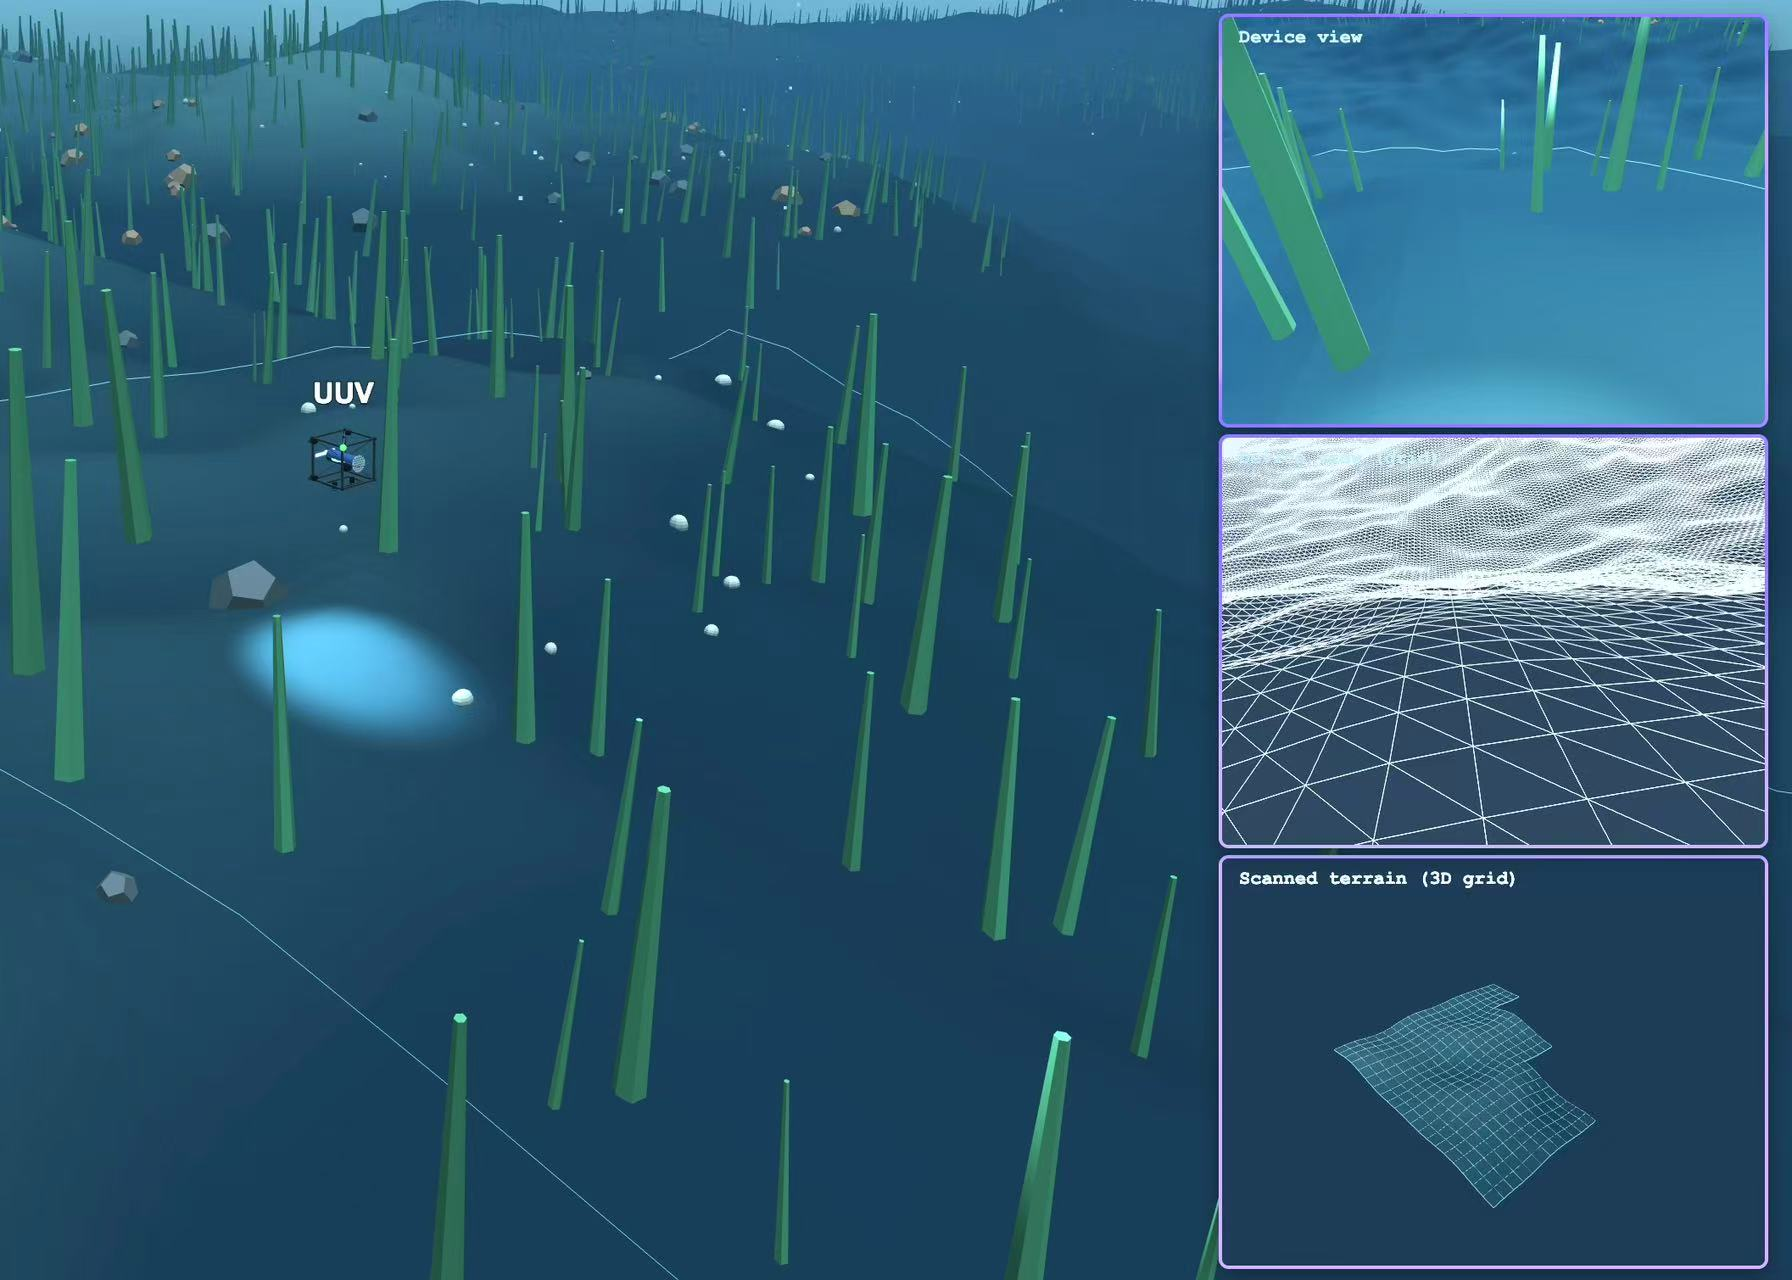
\includegraphics[width=0.48\linewidth]{figures/task4_ui_off.png}}
 \hfill
 \subfloat[FH: Fish Protection / Herding (8 UUVs)]{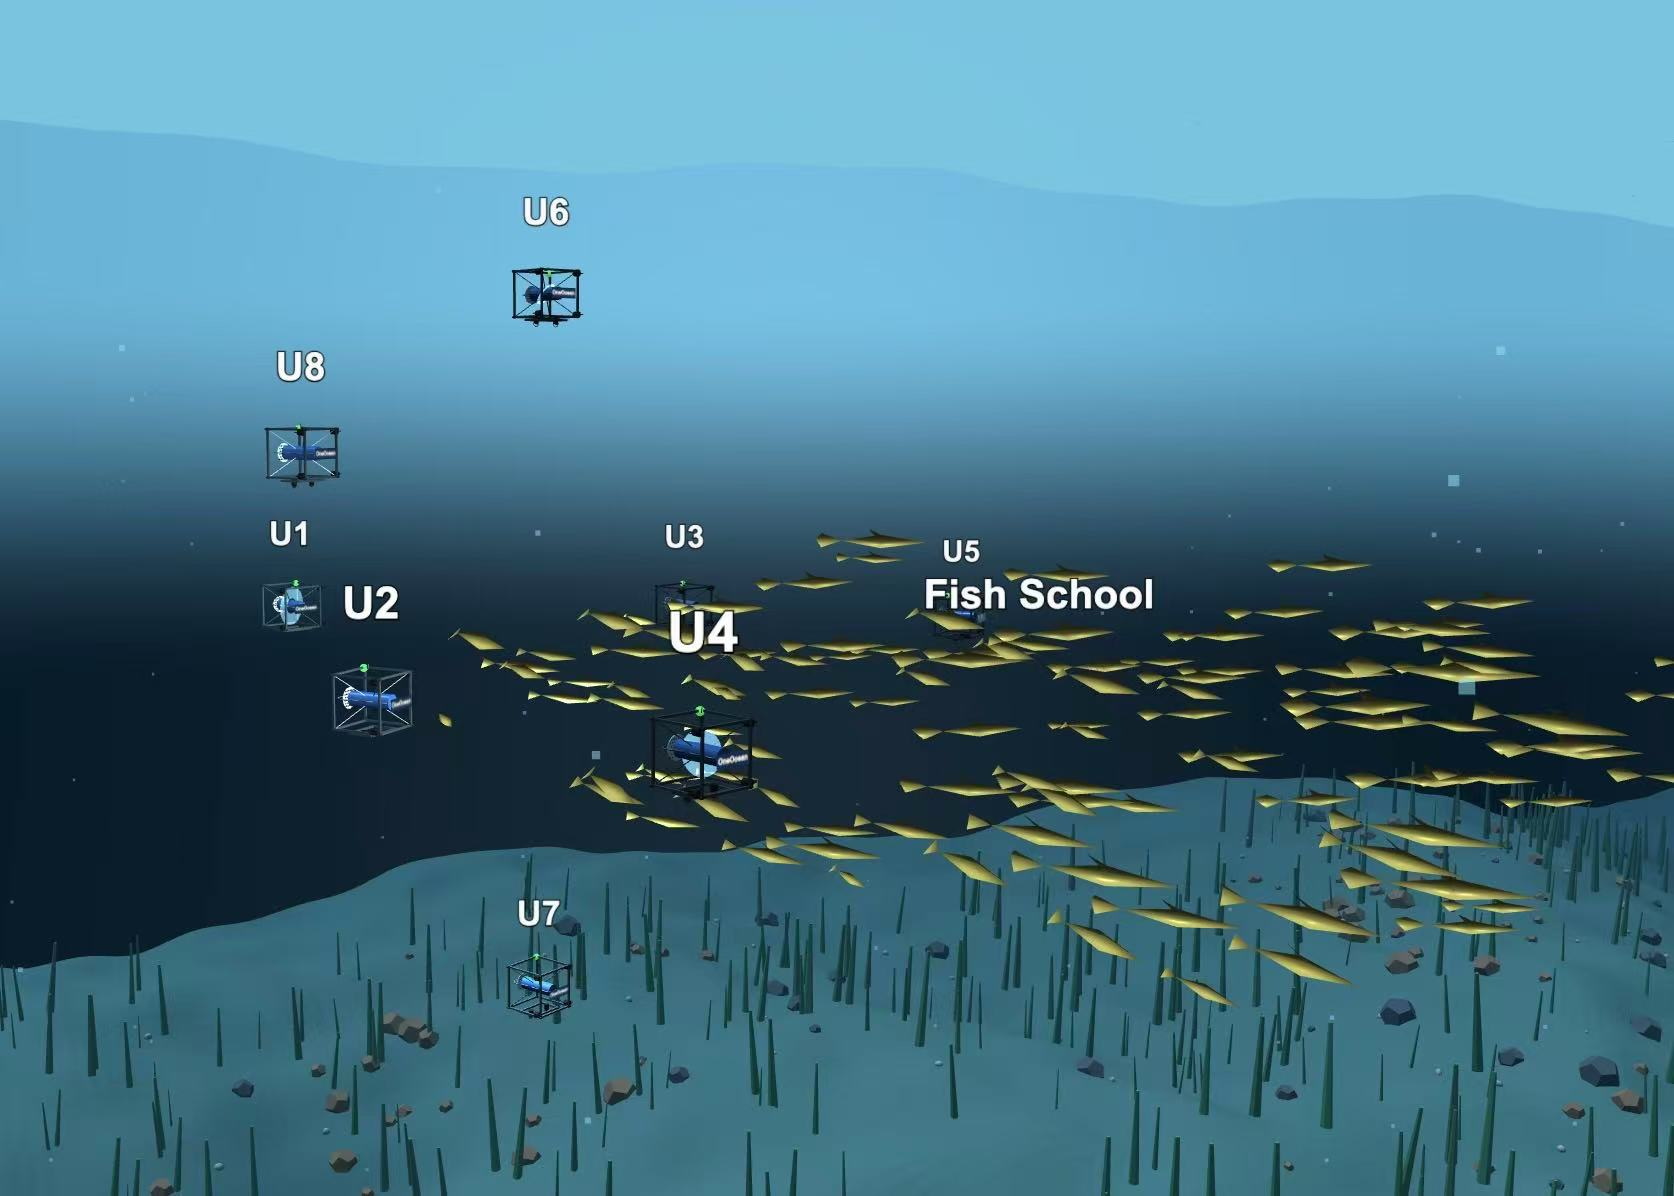
\includegraphics[width=0.48\linewidth]{figures/task3_ui_off.png}}
 \caption{Surface Pollution Cleanup, Underwater Pollution Lift, Area Scan, and Fish Protection / Herding in the core backend.}
 \label{fig:core_ui_off_panel}
\end{figure}
}


\revise{
\begin{table}[t]
\centering
\scriptsize
\setlength{\tabcolsep}{1.2pt}
\renewcommand{\arraystretch}{1.10}
\begin{tabularx}{\columnwidth}{@{}>{\raggedright\arraybackslash}p{0.26\columnwidth}*{7}{Y}@{}}
\toprule
\textbf{Method} & \makecell{\textbf{Avg.}\\\textbf{SR(\%)}} & \makecell{\textbf{Calls}} & \makecell{\textbf{Lat.}\\\textbf{(s)}} & \makecell{\textbf{ms per}\\\textbf{call}} & \makecell{\textbf{Prompt}\\\textbf{tok.}} & \makecell{\textbf{Output}\\\textbf{tok.}} & \makecell{\textbf{Total}\\\textbf{tok.}} \\
\midrule
\rowcolor{oursbg}
LLM-Qwen2.5-7B & \best{65.0} & 6.48 & 14.21 & 2222.1 & 3932 & 4084 & 8016 \\
LLM-Qwen2-7B & 53.3 & \best{4.71} & 11.24 & 2440.3 & 2877 & 2996 & 5873 \\
LLM-Mistral-7B & 53.3 & 6.05 & 31.38 & 4942.5 & 3762 & 4128 & 7890 \\
LLM-ChatGLM3-6B & 53.3 & 5.38 & \best{7.91} & \best{1393.6} & 3414 & \best{411} & \best{3825} \\
\rowcolor{oursbg}
Heuristic & 55.0 & \best{0.00} & \best{0.00} & \best{0.0} & \best{0} & \best{0} & \best{0} \\
LLM-Llama3-8B & 45.0 & 6.71 & 13.94 & 2117.5 & 3072 & 3218 & 6292 \\
LLM-Llama2-7B & 33.3 & 6.59 & 49.42 & 7401.8 & 4219 & 4851 & 9071 \\
BC & 21.7 & \best{0.00} & \best{0.00} & \best{0.0} & \best{0} & \best{0} & \best{0} \\
\bottomrule
\end{tabularx}
\caption{Core-benchmark planning-suite cost metrics at Tier 2 with doubled currents: uncached local-inference calls, latency, and token usage, reported alongside average success over 20 episodes per task.}
\label{tab:planning_suite_cost_t2}
\end{table}
}

\revise{Across ten tasks, heuristic success decreases from 84.6\% at Tier 2 to 29.0\% at Tier 3, while BC decreases from 58.6\% to 6.0\% (Table~\ref{tab:headline_macro_keymetrics}). Table~\ref{tab:per_task_sr_t2_t3} reports the task-level changes, including gaps in Station Keeping, Route Following, Surface Pollution Cleanup, and Pipeline Inspection. Figure~\ref{fig:core_ui_off_panel} shows four tasks from the suite.}

\revise{Figure~\ref{fig:difficulty_ladder_dualpanel} compares success across all three tiers for a five-task subset.}

\revise{
\begin{figure*}[t]
 \centering
 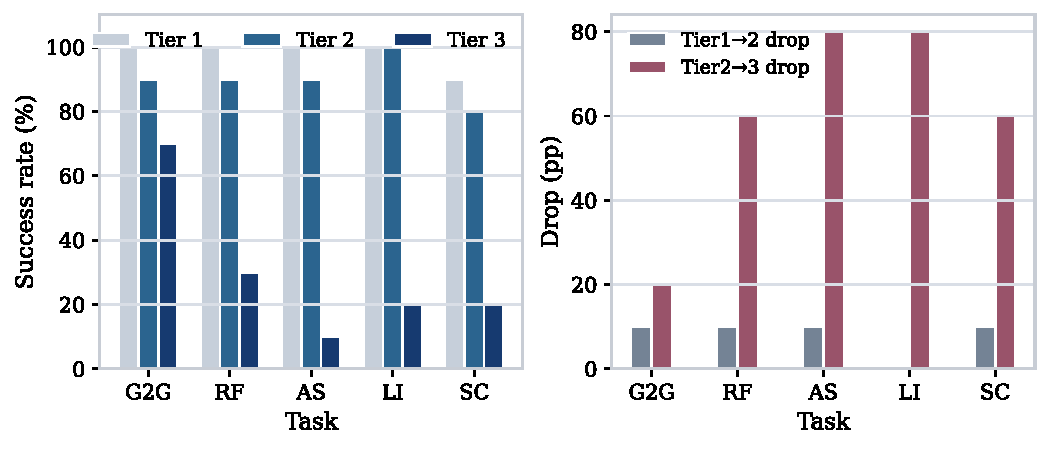
\includegraphics[width=0.98\textwidth]{figures/difficulty_ladder_dualpanel.pdf}
 \caption{Success rates across difficulty tiers for a five-task subset. Left: success rate at Tiers~1--3. Right: success-rate drops from Tier~1$\rightarrow$2 and Tier~2$\rightarrow$3.}
 \label{fig:difficulty_ladder_dualpanel}
\end{figure*}
}

\revise{Heuristic control has higher macro success at both tiers. BC performs well on \emph{Underwater Pollution Lift (UPL)} and \emph{Fish Protection / Herding (FH)} at Tier 2, but declines on tasks requiring persistent disturbance rejection or coordinated geometry. In Surface Pollution Cleanup, larger teams improve success and source completion while increasing collision exposure (Figure~\ref{fig:cleanup_scaling_dualpanel}). The action-energy proxy varies non-monotonically with team size.}

\paragraph{Planning-sensitive tasks.}

\revise{We compare deterministic heuristic control, BC, and local LLM planners on Surface Pollution Cleanup (SPC), Area Scan (AS), and Pipeline Inspection (PI). Each LLM proposes assignments or waypoints at a fixed stride; a deterministic controller executes them with shared safety checks.}

\revise{In the 40-episode-per-task study, heuristic control has the highest average success (Table~\ref{tab:planning_suite_perf_t2}). ChatGLM3-6B matches its cleanup rate and achieves the highest scan coverage. In the separate 20-episode-per-task cost study, Qwen2.5-7B has the highest average success, and ChatGLM3-6B has the lowest LLM inference latency (Table~\ref{tab:planning_suite_cost_t2}).}

\revise{In the three-seed planning diagnostic, valid plans can revisit covered cells or miss leaks, while invalid responses invoke the deterministic task allocator. We report executed command effort through $E$ and inference cost through latency and token counts. Appendix Sec.~\ref{supp-app:core_diagnostics} reports task-level and model-level validity, fallback, completion, token, and latency values.}

\revise{
\begin{figure*}[t]
 \centering
 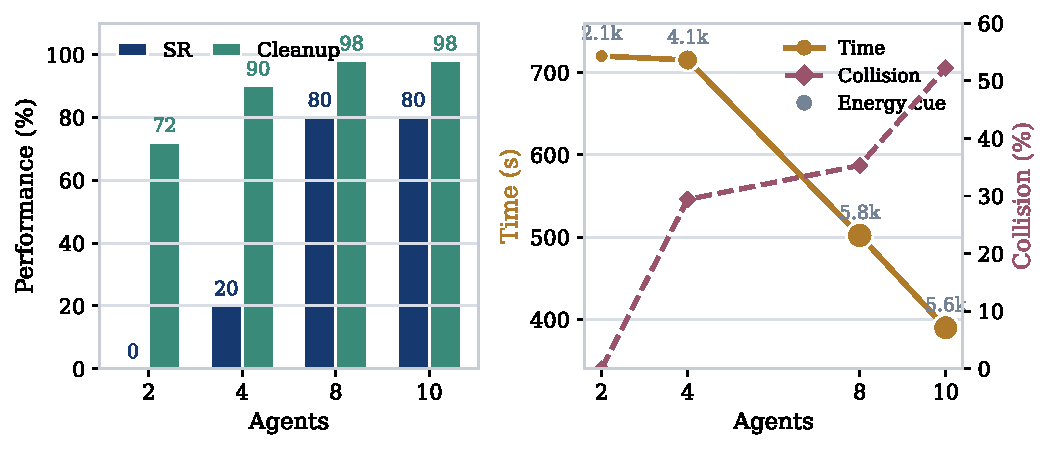
\includegraphics[width=0.98\textwidth]{figures/cleanup_scaling_dualpanel.pdf}
 \caption{Surface-cleanup scaling at Tier~2. Left: success rate and cleanup rate as the number of vehicles increases. Right: completion time and near-collision ratio, with per-point annotations showing the energy proxy in thousands.}
 \label{fig:cleanup_scaling_dualpanel}
\end{figure*}
}

\subsection{External underwater-scene backend}

\revise{
\begin{figure}[ht]
 \centering
 \subfloat[Surface pollution containment and cleanup in a packaged ocean scene.]{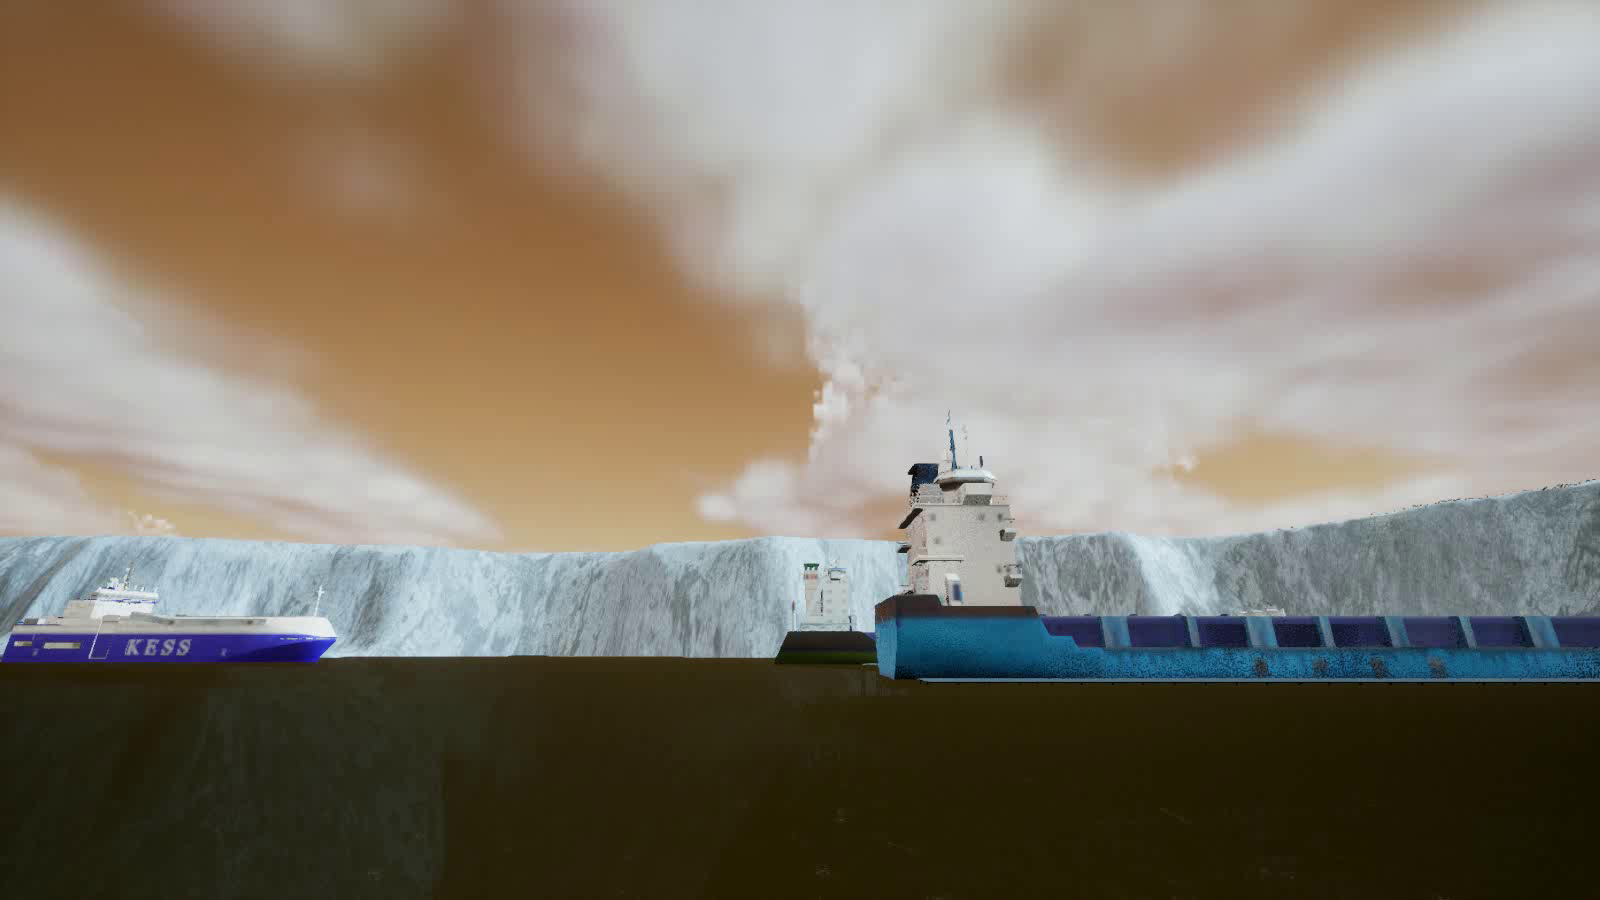
\includegraphics[width=0.48\linewidth]{figures/h3_oceangym_image1_containment.jpg}}
 \hfill
 \subfloat[Multi-agent scene-backed deployment.]{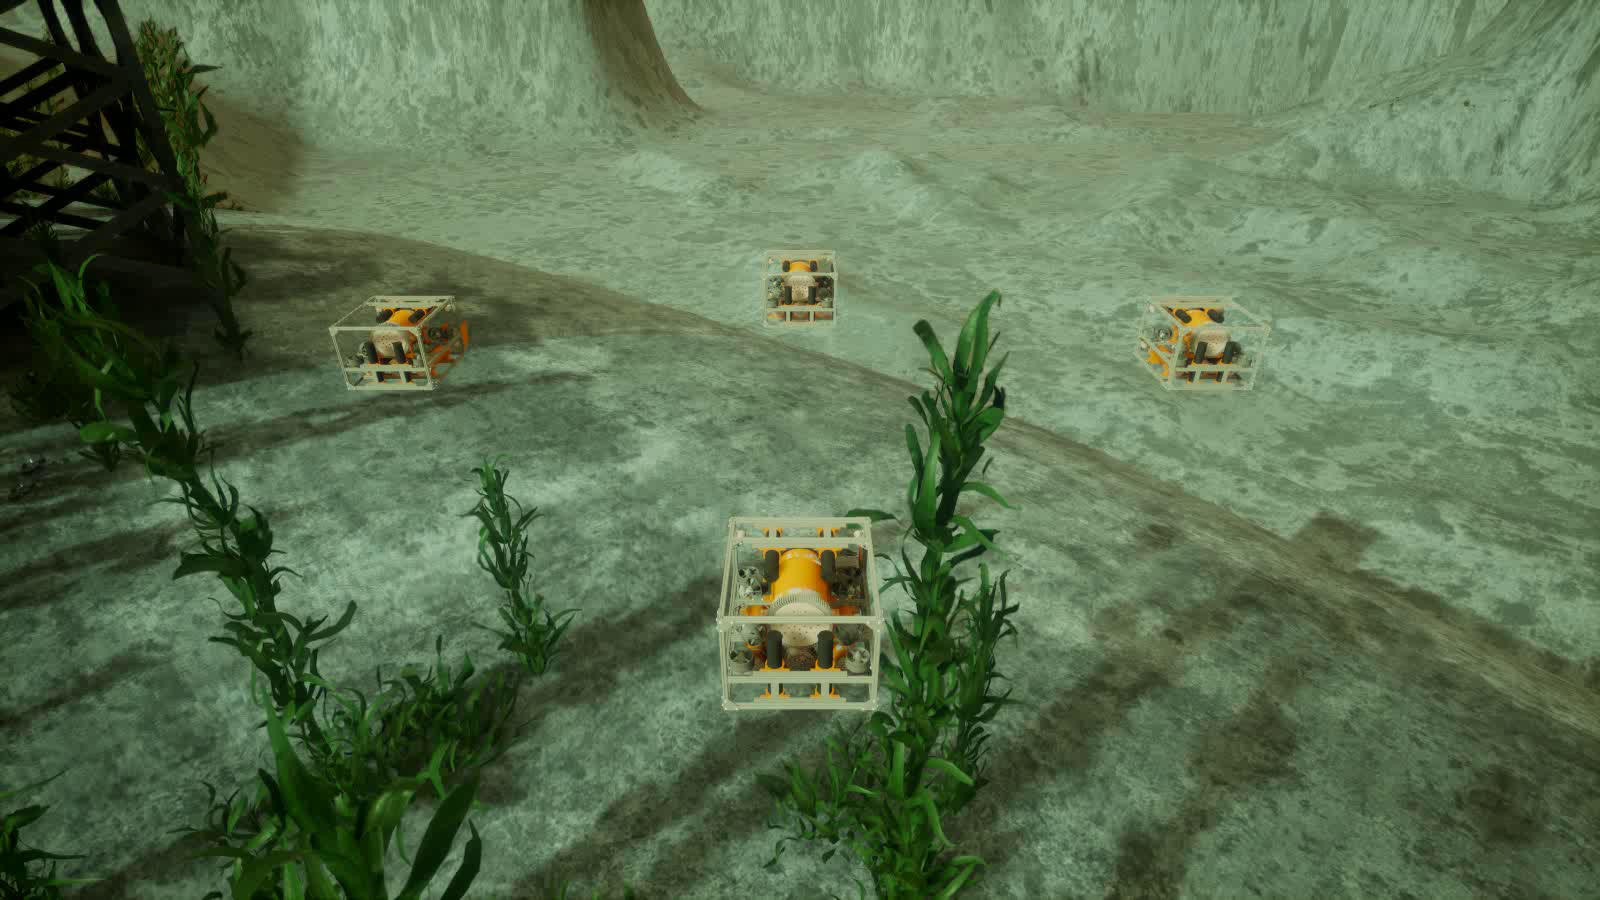
\includegraphics[width=0.48\linewidth]{figures/h3_oceangym_image2_formation.jpg}}
 \caption{Task demonstrations in packaged underwater scenes using currents exported from the OneOcean dataset.}
 \label{fig:extscene_keyframes}
\end{figure}
}

\revise{Route-following performance varies across four underwater scenes (Table~\ref{tab:h3_route_generalization}), while Figure~\ref{fig:extscene_keyframes} shows pollution-response and multi-agent demonstrations. The scene backend introduces scene geometry and applies currents through a one-way disturbance interface. A separate diagnostic found lower localization error with OCPNet-3D under both tested current settings, with aggregate success matching or exceeding the analytic probe. Appendix Sec.~\ref{supp-app:external_diagnostics} provides the values and episode budgets.}

\revise{
\begin{table}[t]
\centering
\scriptsize
\setlength{\tabcolsep}{1.2pt}
\renewcommand{\arraystretch}{1.12}
\begin{tabularx}{\columnwidth}{@{}>{\raggedright\arraybackslash}p{0.25\columnwidth}*{6}{Y}@{}}
\toprule
\multirow{2}{*}{\textbf{Scene}} & \multicolumn{3}{c}{\textbf{Tier 2}} & \multicolumn{3}{c}{\textbf{Tier 3}} \\
\cmidrule(lr){2-4}\cmidrule(lr){5-7}
 & \makecell{SR\\(\%)} & \makecell{WP} & \makecell{CTE\\(m)} & \makecell{SR\\(\%)} & \makecell{WP} & \makecell{CTE\\(m)} \\
\midrule
Dam & 0.0 & 1.0 & 3.06 & 0.0 & 0.0 & \best{0.87} \\
OpenWater & 20.0 & 3.1 & 2.50 & 0.0 & 0.0 & 1.91 \\
PierHarbor & 56.7 & 3.5 & \best{2.22} & 0.0 & 2.0 & 1.41 \\
SimpleUnderw. & \best{100.0} & \best{4.0} & 3.04 & \best{96.7} & \best{3.0} & 2.16 \\
\rowcolor{scenarioGray}
Mean over scenes & 44.2 & 2.92 & 2.70 & 24.2 & 1.25 & 1.59 \\
\bottomrule
\end{tabularx}
\caption{Route-following across four underwater scenes, with 30 episodes per difficulty in each scene. WP denotes the mean number of reached waypoints; CTE denotes Cross-Track Error.}
\label{tab:h3_route_generalization}
\end{table}
}

\section{Discussion}
\label{sec:discussion}

\revise{Heuristic control achieves higher macro success than BC across the ten-task suite, while BC performs well on Underwater Pollution Lift and Fish Protection / Herding at Tier 2. Stronger currents and tighter task requirements expose failures in sustained tracking and coordination. LLM performance varies across tasks and evaluation sweeps, with latency and token usage adding to the cost of planning.}

\revise{Task-specific progress, command effort, collision exposure, and completion time complement binary success. The planner diagnostics connect task outcomes to plan validity and fallback behavior. Valid assignments can yield poor trajectories or repeated coverage, while invalid calls invoke the deterministic allocator. These observations emphasize the role of closed-loop execution when evaluating high-level planning.}

\revise{The external experiments show scene-dependent route-following performance under the shared task definitions. Core episodes use fixed current slices, while scene episodes use temporal forcing and scene-specific geometry. Recording these settings supports comparisons across environments and helps identify which conditions challenge a controller.}

\section{Conclusion}
\revise{OneOcean combines a shared ocean dataset, ten marine-robotics tasks, and a standardized evaluation protocol. Its headless and underwater-scene backends support reproducible experiments under data-grounded disturbances. The experiments compare task performance, robustness to currents, planning cost, and transfer across underwater scenes. Future work will improve tide coupling and three-dimensional currents and broaden the tasks and robot morphologies.}


\clearpage
\bibliography{references}

\end{document}
